\section{Problema inicial}
En la figura %\ref{fig:problem} 
se muestra el problema asignado a este grupo de trabajo.
Este consiste en dos eslabones articulados en un mismo punto, llamado $B$; cuyos
extremos libres, Punto $C$ y punto $A$, son empujados por dos actuadores lineales en
direcciones paralelas con velocidades dadas $v_A$ y $v_C$.

\begin{figure}[!h]
	\centering
	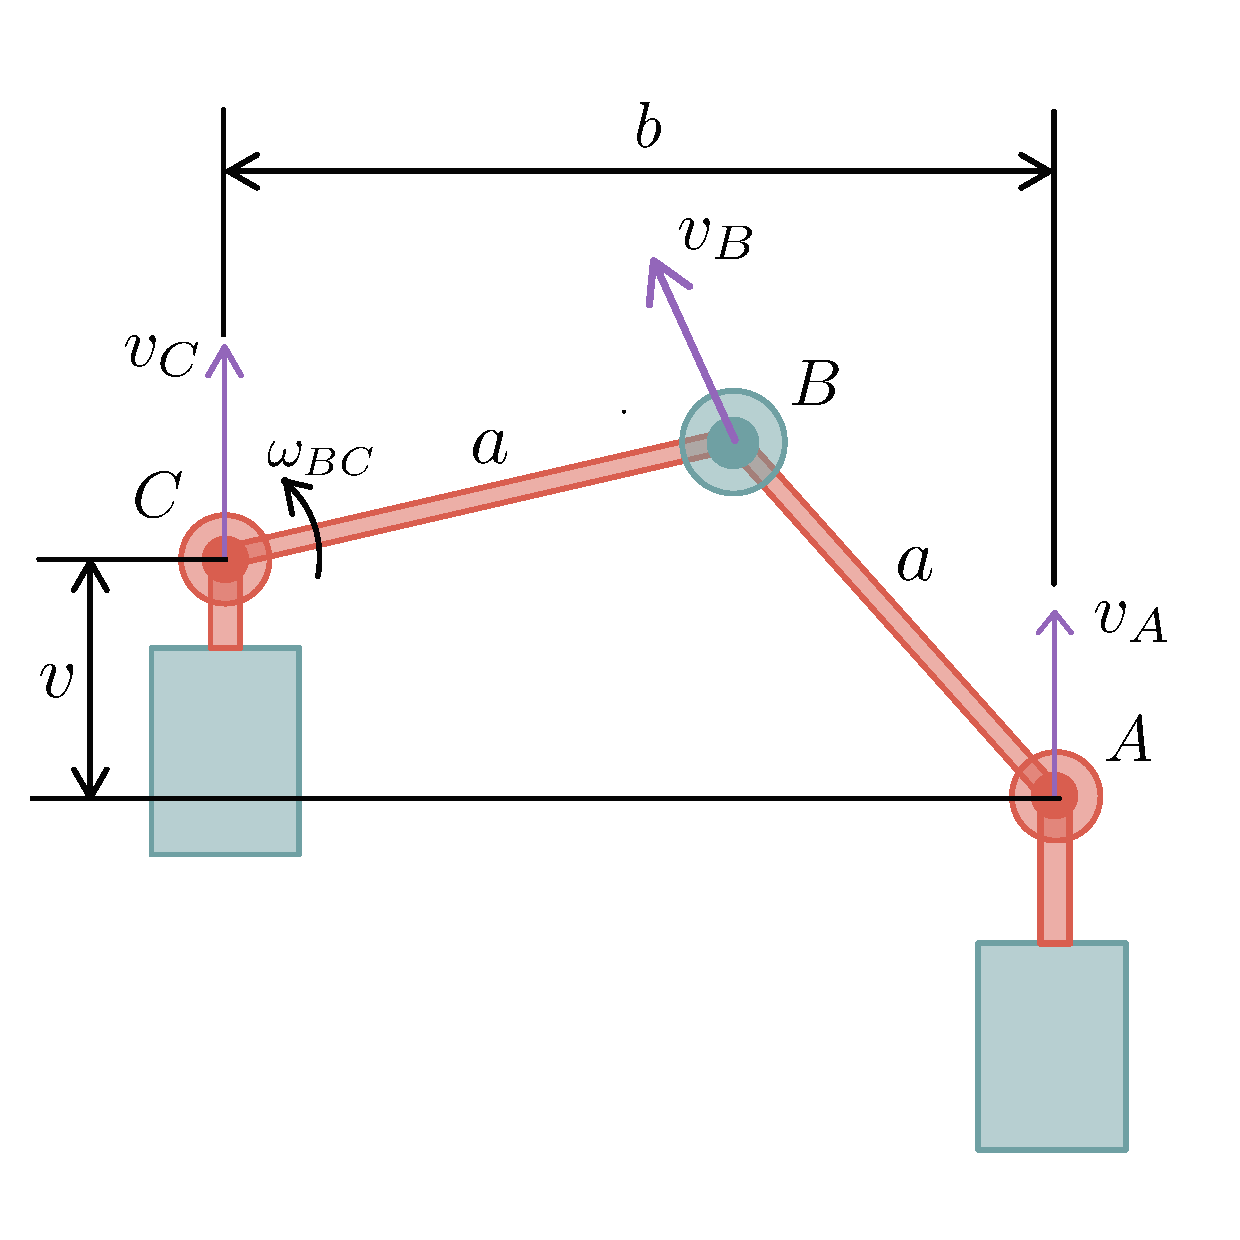
\includegraphics[height=8cm]{img/problem.pdf}
	\caption{Mecanismo planteado.}
	\label{fig:problem}
\end{figure}

Mediante un análisis vectorial, se desea determinar la posición, velocidad y
aceleración del punto \(B\), así como la velocidad angular del eslabón \(CB\). Se
consideran conocidas las longitudes \(v\), \(b\) y \(a\), junto con las velocidades
\(v_C\) y \(v_A\). Por conveniencia, para la construcción del mecanismo, se adoptan los
siguientes valores:

\[
v = 150\,\text{mm}, \qquad b = 250\,\text{mm}, \qquad a = 200\,\text{mm}
\]

\[
v_C = 30\,\text{mm/s}, \qquad v_A = 20\,\text{mm/s}
\]

Quedan por determinar:
\[
\overrightarrow{r}_B,\quad \overrightarrow{v}_B,\quad \overrightarrow{a}_B,\quad \omega_{BC}
\]
% \section{Problema inicial}
En la figura %\ref{fig:problem} 
se muestra el problema asignado a este grupo de trabajo.
Este consiste en dos eslabones articulados en un mismo punto, llamado $B$; cuyos
extremos libres, Punto $C$ y punto $A$, son empujados por dos actuadores lineales en
direcciones paralelas con velocidades dadas $v_A$ y $v_C$.

\begin{figure}[!h]
	\centering
	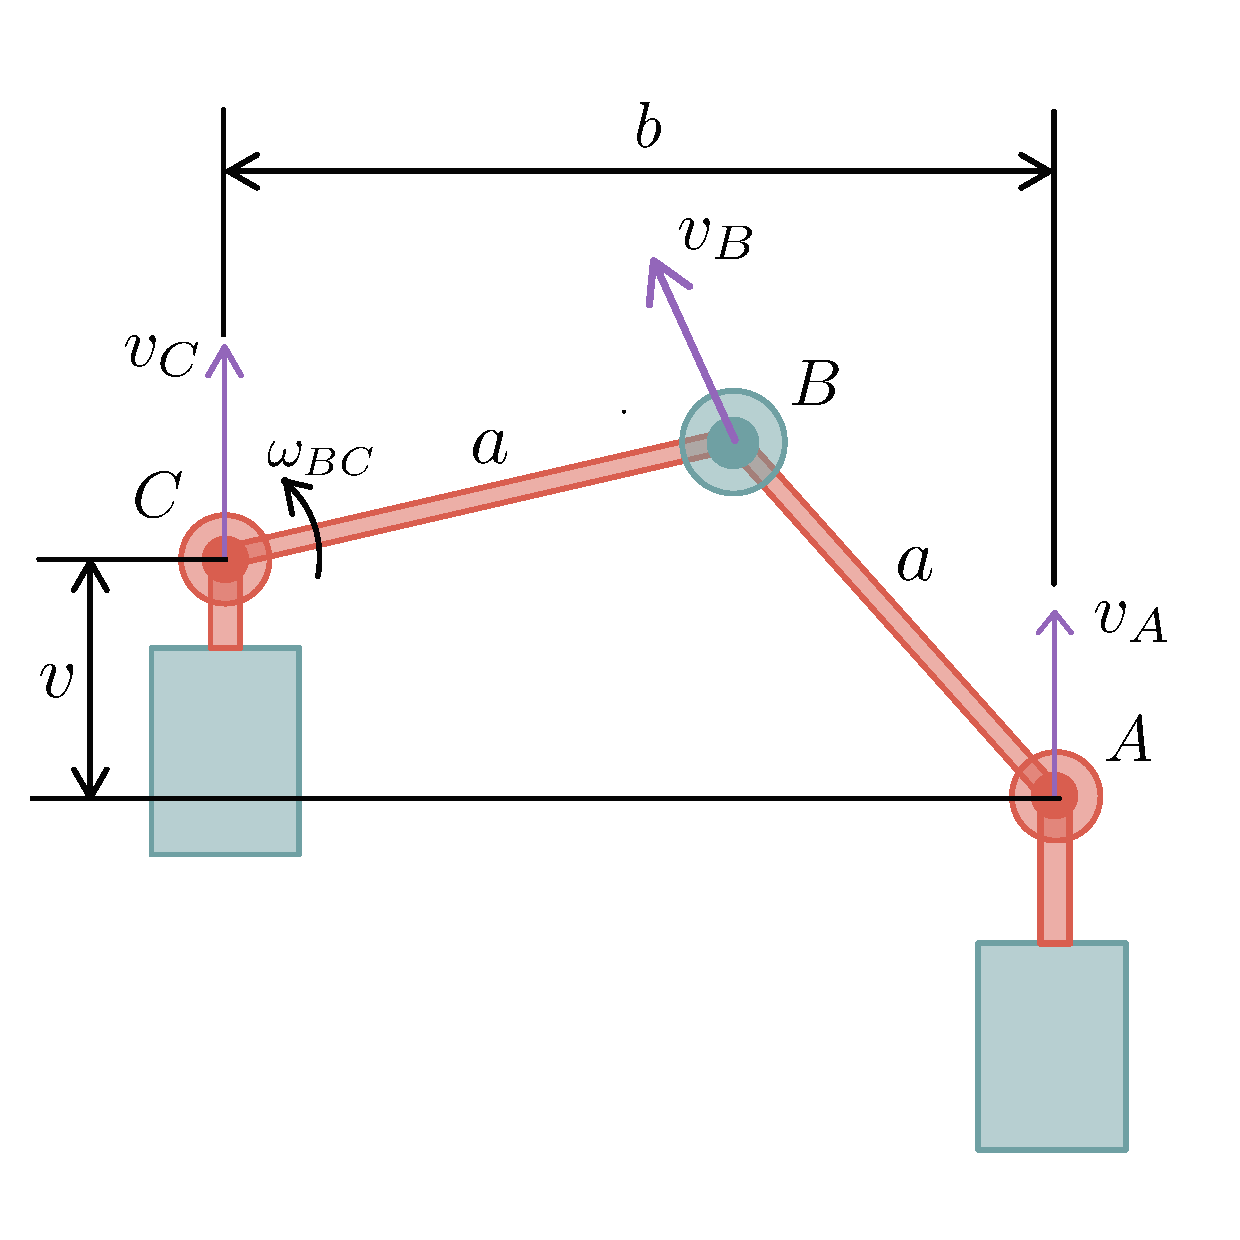
\includegraphics[height=8cm]{img/problem.pdf}
	\caption{Mecanismo planteado.}
	\label{fig:problem}
\end{figure}

Mediante un análisis vectorial, se desea determinar la posición, velocidad y
aceleración del punto \(B\), así como la velocidad angular del eslabón \(CB\). Se
consideran conocidas las longitudes \(v\), \(b\) y \(a\), junto con las velocidades
\(v_C\) y \(v_A\). Por conveniencia, para la construcción del mecanismo, se adoptan los
siguientes valores:

\[
v = 150\,\text{mm}, \qquad b = 250\,\text{mm}, \qquad a = 200\,\text{mm}
\]

\[
v_C = 30\,\text{mm/s}, \qquad v_A = 20\,\text{mm/s}
\]

Quedan por determinar:
\[
\overrightarrow{r}_B,\quad \overrightarrow{v}_B,\quad \overrightarrow{a}_B,\quad \omega_{BC}
\]
% \section{Problema inicial}
En la figura %\ref{fig:problem} 
se muestra el problema asignado a este grupo de trabajo.
Este consiste en dos eslabones articulados en un mismo punto, llamado $B$; cuyos
extremos libres, Punto $C$ y punto $A$, son empujados por dos actuadores lineales en
direcciones paralelas con velocidades dadas $v_A$ y $v_C$.

\begin{figure}[!h]
	\centering
	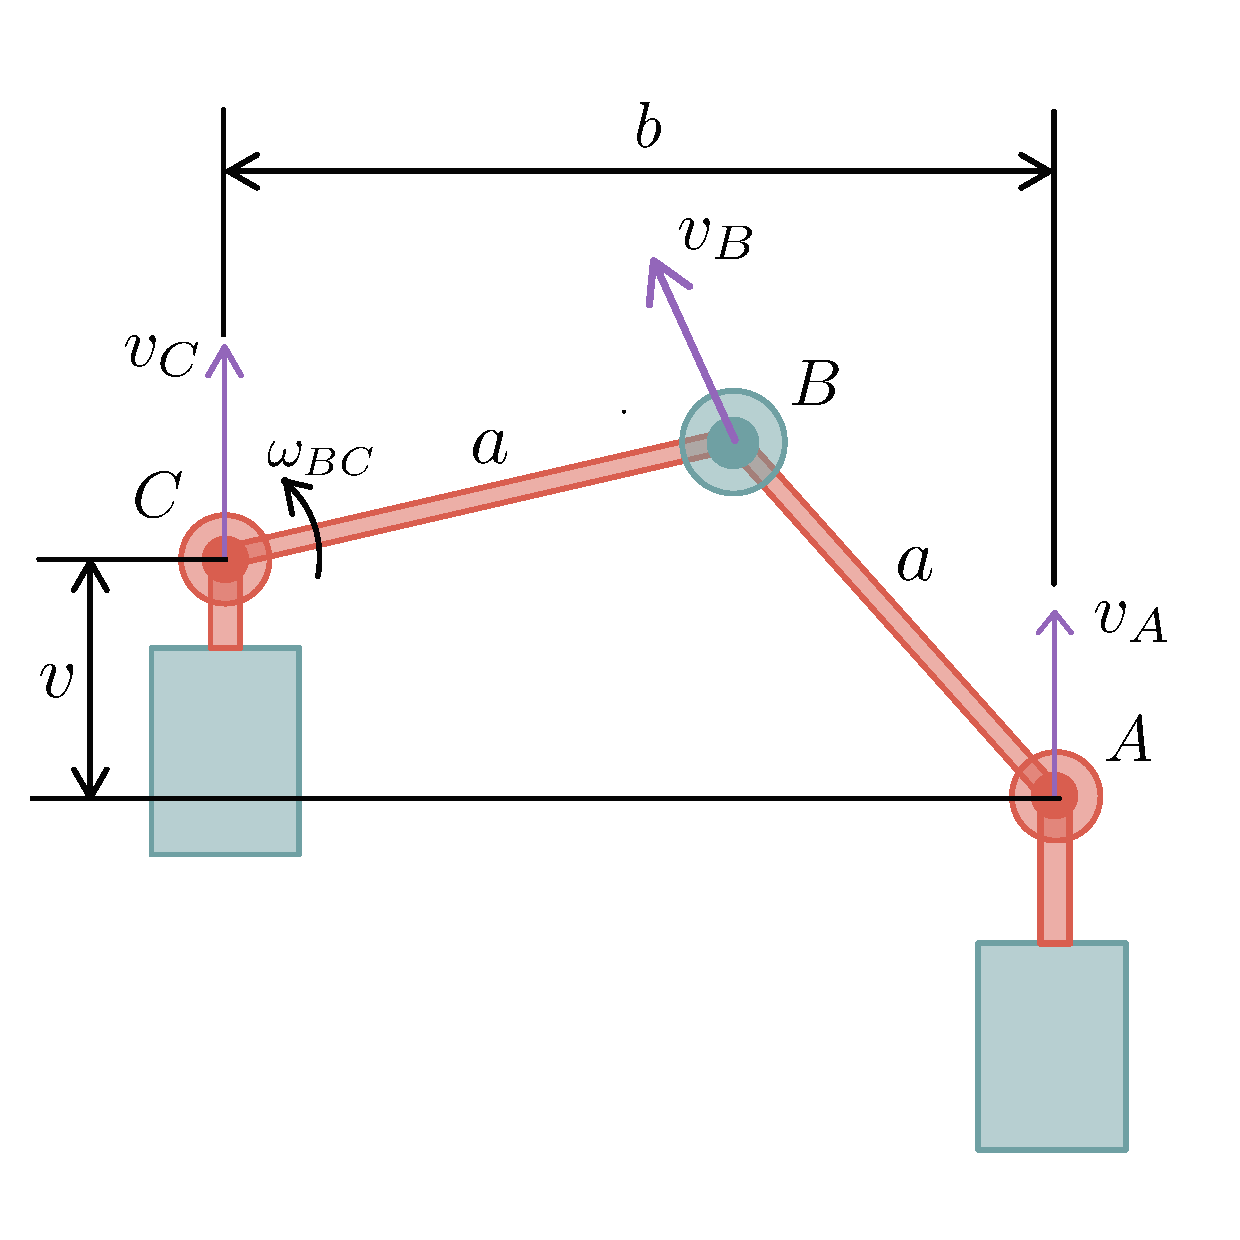
\includegraphics[height=8cm]{img/problem.pdf}
	\caption{Mecanismo planteado.}
	\label{fig:problem}
\end{figure}

Mediante un análisis vectorial, se desea determinar la posición, velocidad y
aceleración del punto \(B\), así como la velocidad angular del eslabón \(CB\). Se
consideran conocidas las longitudes \(v\), \(b\) y \(a\), junto con las velocidades
\(v_C\) y \(v_A\). Por conveniencia, para la construcción del mecanismo, se adoptan los
siguientes valores:

\[
v = 150\,\text{mm}, \qquad b = 250\,\text{mm}, \qquad a = 200\,\text{mm}
\]

\[
v_C = 30\,\text{mm/s}, \qquad v_A = 20\,\text{mm/s}
\]

Quedan por determinar:
\[
\overrightarrow{r}_B,\quad \overrightarrow{v}_B,\quad \overrightarrow{a}_B,\quad \omega_{BC}
\]
% \section{Problema inicial}
En la figura %\ref{fig:problem} 
se muestra el problema asignado a este grupo de trabajo.
Este consiste en dos eslabones articulados en un mismo punto, llamado $B$; cuyos
extremos libres, Punto $C$ y punto $A$, son empujados por dos actuadores lineales en
direcciones paralelas con velocidades dadas $v_A$ y $v_C$.

\begin{figure}[!h]
	\centering
	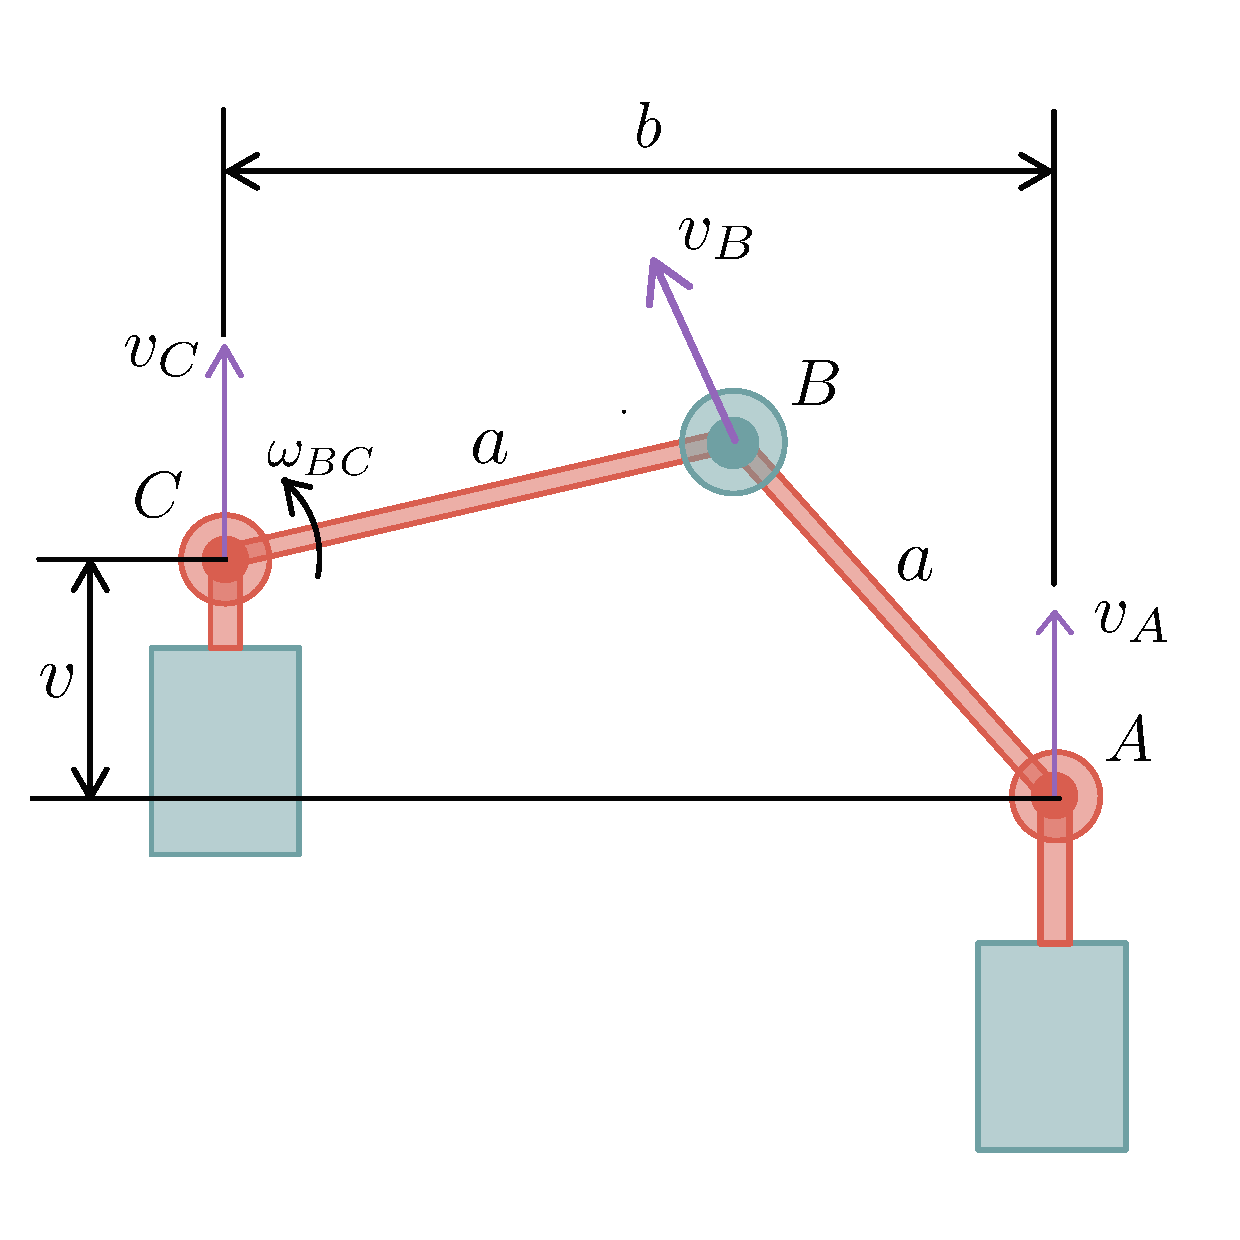
\includegraphics[height=8cm]{img/problem.pdf}
	\caption{Mecanismo planteado.}
	\label{fig:problem}
\end{figure}

Mediante un análisis vectorial, se desea determinar la posición, velocidad y
aceleración del punto \(B\), así como la velocidad angular del eslabón \(CB\). Se
consideran conocidas las longitudes \(v\), \(b\) y \(a\), junto con las velocidades
\(v_C\) y \(v_A\). Por conveniencia, para la construcción del mecanismo, se adoptan los
siguientes valores:

\[
v = 150\,\text{mm}, \qquad b = 250\,\text{mm}, \qquad a = 200\,\text{mm}
\]

\[
v_C = 30\,\text{mm/s}, \qquad v_A = 20\,\text{mm/s}
\]

Quedan por determinar:
\[
\overrightarrow{r}_B,\quad \overrightarrow{v}_B,\quad \overrightarrow{a}_B,\quad \omega_{BC}
\]
% \input{sections/marco_teorico}  % Eliminada inclusión recursiva (causaba bucle)
\subsection{Cinemática básica}
La cinemática es la parte de la mecánica que estudia el movimiento de los cuerpos sin
preocuparse por qué lo causan, es decir, sin importar fuerzas ni masas. Lo que interesa
aquí son las variables geométricas: posición, velocidad y aceleración en función del tiempo.
\\
\subsubsection{Posición y desplazamiento}

La posición de un punto en el plano se describe con un vector $\vec{r}$ que va desde el
origen del sistema de referencia hasta ese punto:

\begin{equation}
	\vec{r} = x\,\hat{i} + y\,\hat{j}
\end{equation}

El desplazamiento entre dos posiciones es simplemente la diferencia:

\begin{equation}
	\Delta\vec{r} = \vec{r}_2 - \vec{r}_1 = (x_2 - x_1)\,\hat{i} + (y_2 - y_1)\,\hat{j}
\end{equation}

En el mecanismo, los puntos $A$, $B$ y $C$ se ubican así en el plano. El punto $B$ es el
que queremos encontrar a partir de las posiciones que los actuadores imponen en $A$ y $C$.
\\
\subsubsection{Velocidad}

La velocidad es la derivada de la posición respecto al tiempo:

\begin{equation}
	\vec{v} = \frac{d\vec{r}}{dt} = \dot{x}\,\hat{i} + \dot{y}\,\hat{j}
\end{equation}

Su magnitud (la rapidez) es:

\begin{equation}
	|\vec{v}| = \sqrt{v_x^2 + v_y^2}
\end{equation}

En nuestro caso, las velocidades de $A$ y $C$ son conocidas y verticales:
$\vec{v}_A = 20\,\text{mm/s}\,\hat{j}$ y $\vec{v}_C = 30\,\text{mm/s}\,\hat{j}$.
Lo que se quiere encontrar es $\vec{v}_B$.

\subsubsection{Aceleración}

La aceleración es la derivada de la velocidad:

\begin{equation}
	\vec{a} = \frac{d\vec{v}}{dt} = \ddot{x}\,\hat{i} + \ddot{y}\,\hat{j}
\end{equation}

Cuando un punto describe una trayectoria curvilínea, la aceleración tiene dos componentes:
una tangencial (que cambia qué tan rápido va) y una normal o centrípeta (que cambia hacia
dónde va):

\begin{equation}
	\vec{a} = a_t\,\hat{e}_t + a_n\,\hat{e}_n
\end{equation}

La componente centrípeta para movimiento circular vale:

\begin{equation}
	a_n = \omega^2 \cdot r
\end{equation}

donde $\omega$ es la velocidad angular y $r$ la distancia al centro de rotación.
Esto aplica directamente al punto $B$, que sigue una trayectoria curvilínea al estar
conectado a los dos eslabones.

% ------------------------------------------------
\subsection{Cinemática de cuerpos rígidos}

Un cuerpo rígido es aquel en el que la distancia entre cualquier par de sus puntos no
cambia durante el movimiento. Gracias a esto, se puede extender el análisis de una partícula
a todo el cuerpo usando unas pocas ecuaciones.
\\
\subsubsection{Movimiento plano general}

El movimiento plano de un cuerpo rígido siempre se puede separar en una traslación (que
lleva un punto de referencia a su nueva posición) más una rotación alrededor de ese punto.
En general:

\begin{align} 
	\vec{r}_B &= \vec{r}_A + \vec{r}_{B/A} \label{eq:pos_rel} \\
	\vec{v}_B &= \vec{v}_A + \vec{v}_{B/A} \label{eq:vel_rel} \\
	\vec{a}_B &= \vec{a}_A + \vec{a}_{B/A} \label{eq:acc_rel} 
\end{align}

\subsubsection{Ecuación de velocidad relativa}

La velocidad de $B$ relativa a $A$, cuando el cuerpo rota con velocidad angular $\omega$,
se calcula con el producto vectorial:

\begin{equation}
	\vec{v}_{B/A} = \vec{\omega} \times \vec{r}_{B/A}
\end{equation}

Con $\vec{\omega} = \omega\,\hat{k}$ y $\vec{r}_{B/A} = r_x\,\hat{i} + r_y\,\hat{j}$,
el resultado en el plano es:

\begin{equation}
	\vec{v}_{B/A} = -\omega r_y\,\hat{i} + \omega r_x\,\hat{j}
\end{equation}

Aplicada al eslabón $CB$ del mecanismo:

\begin{equation}
	\vec{v}_B = \vec{v}_C + \vec{\omega}_{BC} \times \vec{r}_{B/C}
	\label{eq:vel_eslabon}
\end{equation}

Esta ecuación vectorial equivale a dos ecuaciones escalares (componentes $x$ e $y$), con
las que se pueden encontrar las dos incógnitas: las componentes de $\vec{v}_B$ y la
velocidad angular $\omega_{BC}$.
\\
\subsubsection{Ecuación de aceleración relativa}

La aceleración relativa tiene dos partes: la tangencial (por cambio en $\omega$) y la
centrípeta (por cambio de dirección):

\begin{equation}
	\vec{a}_{B/A} = \vec{\alpha} \times \vec{r}_{B/A} - \omega^2\,\vec{r}_{B/A}
\end{equation}

donde $\alpha = \dot{\omega}$ es la aceleración angular. La aceleración total de $B$ queda:

\begin{equation}
	\vec{a}_B = \vec{a}_A + \vec{\alpha} \times \vec{r}_{B/A} - \omega^2\,\vec{r}_{B/A}
\end{equation}

Para el eslabón $CB$:

\begin{equation}
	\vec{a}_B = \vec{a}_C + \alpha_{BC}\,\hat{k} \times \vec{r}_{B/C}
	- \omega_{BC}^2\,\vec{r}_{B/C}
	\label{eq:acc_eslabon}
\end{equation}

De nuevo, dos ecuaciones escalares que permiten hallar $\vec{a}_B$ y $\alpha_{BC}$,
una vez conocida $\omega_{BC}$ del paso anterior.
\\
\subsubsection{Lazo vectorial de cierre}

Para encontrar la posición de $B$ a partir de la geometría del mecanismo, se plantea
la ecuación de cierre del lazo:

\begin{equation}
	\vec{r}_B = \vec{r}_C + \vec{r}_{B/C} = \vec{r}_A + \vec{r}_{B/A}
\end{equation}

junto con las restricciones de longitud de cada eslabón:

\begin{align}
	|\vec{r}_{B/C}| &= b = 250\,\text{mm} \\
	|\vec{r}_{B/A}| &= a = 200\,\text{mm}
\end{align}

Esto forma un sistema de dos ecuaciones con dos incógnitas ($x_B$, $y_B$) que tiene
solución única para una configuración dada del mecanismo.

% ------------------------------------------------
\subsection{Mecanismo tornillo-tuerca}

Para generar el movimiento lineal de los puntos $A$ y $C$ se optó por un mecanismo
tornillo-tuerca, dado que sus componentes (barra roscada, tuerca y motor) son fácilmente
conseguibles y ofrecen buena precisión sin necesidad de impresión 3D de piezas críticas.

El principio es simple: el motor hace girar la barra roscada, y la tuerca que no puede
girar porque está unida al eslabón avanza linealmente. La relación entre la velocidad
angular del motor $\omega_m$ y la velocidad lineal resultante $v_L$ es:

\begin{equation}
	v_L = \frac{\omega_m \cdot p}{2\pi}
\end{equation}

donde $p$ es el paso del tornillo (avance por vuelta). El par necesario para vencer una
carga axial $F$ con eficiencia $\eta$ es:

\begin{equation}
	T = \frac{F \cdot p}{2\pi\,\eta}
\end{equation}

% ------------------------------------------------
\subsection{Motor paso a paso NEMA 17}

El motor paso a paso es un motor eléctrico que no gira continuamente sino que avanza en
pasos discretos. Cada pulso eléctrico que recibe el driver hace que el rotor se mueva un
ángulo fijo, llamado ángulo de paso $\theta_s$. Para el NEMA 17 genérico usado en este
proyecto, el ángulo de paso típico es de $1.8°$, lo que equivale a 200 pasos por vuelta.

Esto lo hace ideal para este mecanismo porque permite controlar la posición y velocidad
del actuador de forma precisa sin necesidad de un sensor de posición adicional en el motor,
simplemente contando los pulsos enviados:

\begin{equation}
	\theta = N_{pasos} \cdot \theta_s = N_{pasos} \cdot 1.8°
\end{equation}

\begin{equation}
	v_L = \frac{f_{pulsos} \cdot p}{N_{pasos/rev}}
	= \frac{f_{pulsos} \cdot p}{200}
\end{equation}

donde $f_{pulsos}$ es la frecuencia de los pulsos enviados por el microcontrolador.

A diferencia de un motor DC convencional, el motor paso a paso no requiere retroalimentación
para mantener una velocidad constante en régimen normal, ya que sigue fielmente los pulsos
de entrada siempre que la carga no supere el par de retención. Esto simplifica considerablemente
el control del mecanismo.

% ------------------------------------------------
\subsection{Microcontrolador ESP32}

El ESP32 es el cerebro del sistema. Es un microcontrolador de doble núcleo de 240 MHz con
Wi-Fi y Bluetooth integrados, aunque en este proyecto se usa principalmente por su capacidad
de generar señales de control precisas y leer sensores en tiempo real.

Para controlar el motor NEMA 17 se usa la técnica STEP/DIR: el ESP32 envía pulsos digitales
al driver del motor (por ejemplo A4988 o DRV8825) a través del pin STEP, y define la
dirección de giro con el pin DIR. La frecuencia de los pulsos determina la velocidad:

\begin{equation}
	f_{STEP} = \frac{v_L \cdot N_{pasos/rev}}{p}
\end{equation}

El ESP32 también se encarga de leer los acelerómetros vía protocolo I2C y enviar los datos
al computador por comunicación serial (UART) para su posterior procesamiento en Python o MATLAB.

% ------------------------------------------------
\subsection{Acelerómetro BMI160}

El BMI160 es un sensor MEMS (Micro-Electro-Mechanical Systems) de 6 grados de libertad incluye un acelerómetro triaxial y un giroscopio triaxial en el mismo
chip. En este proyecto se usan dos unidades, uno en el punto $B$ y otro en un punto de
referencia, para medir las aceleraciones del mecanismo durante su movimiento.

Su principio de funcionamiento se basa en la deflexión de una masa sísmica microscópica.
Cuando el sensor experimenta una aceleración, la masa se desplaza respecto a la estructura
fija, y ese desplazamiento se convierte en una diferencia de capacitancia que el chip
transforma en un valor digital.

La aceleración medida en unidades digitales (LSB) se convierte a $\text{m/s}^2$ usando
la sensibilidad del sensor, que depende del rango de medición configurado:

\begin{equation}
	a = \frac{\text{valor}_{LSB}}{\text{Sensibilidad}} \cdot g
\end{equation}

Por ejemplo, con rango $\pm 2g$ la sensibilidad es de $16384\,\text{LSB}/g$, y con
$\pm 4g$ es de $8192\,\text{LSB}/g$. Para este mecanismo, dado que las aceleraciones
esperadas son bajas (del orden de pocos $\text{mm/s}^2$), se configura el rango más
sensible ($\pm 2g$) para maximizar la resolución de las mediciones.

La comunicación con el ESP32 se realiza por el bus I2C a una velocidad de hasta 400 kHz.
Como se usan dos BMI160 en el mismo bus, se configuran en direcciones I2C distintas
(0x68 y 0x69) conectando el pin SDO de cada uno a GND o VDD respectivamente.

% ------------------------------------------------
\subsection{Circuito electrónico}

El circuito del prototipo se organiza en tres etapas: control, adquisición de datos y
potencia.
\subsubsection{Etapa de potencia -- Driver del motor paso a paso}

El motor NEMA 17 no se conecta directamente al ESP32 porque requiere corrientes del orden
de 1 A por fase, mucho más de lo que puede entregar un microcontrolador. Por eso se usa
un driver dedicado (A4988 o DRV8825) que actúa como interfaz entre los pulsos lógicos
del ESP32 y la corriente de las bobinas del motor.

El driver regula la corriente máxima por fase mediante un potenciómetro de ajuste. La
corriente de referencia $I_{ref}$ se relaciona con el voltaje en ese pin según:

\begin{equation}
	I_{ref} = \frac{V_{ref}}{8 \cdot R_{sense}} \quad \text{(para A4988)}
\end{equation}

donde $R_{sense}$ es la resistencia de detección de corriente del driver (típicamente
$0.1\,\Omega$ en módulos comerciales).
\subsubsection{Etapa lógica -- Conexiones del ESP32}

El ESP32 opera a 3.3 V en sus pines GPIO, lo cual es directamente compatible con los
niveles lógicos del driver de motor y del BMI160. Las conexiones principales son:

\begin{itemize}
	\item \textbf{STEP / DIR} del driver: conectados a dos GPIO del ESP32 por cada motor.
	\item \textbf{SDA / SCL} (I2C): bus compartido entre los dos BMI160 y el ESP32
	(pines GPIO 21 y GPIO 22 por defecto en ESP32).
	\item \textbf{ENABLE} del driver: activo en bajo; se mantiene en LOW para habilitar
	el motor durante la operación.
\end{itemize}
\subsubsection{Alimentación}


El circuito necesita dos niveles de tensión:

\begin{itemize}
	\item $3.3\,\text{V}$ para el ESP32 y los sensores BMI160 (regulado internamente
	por el módulo ESP32).
	\item $12\,\text{V}$ (o el voltaje nominal del NEMA 17) para la etapa de potencia
	del driver.
\end{itemize}

Es importante separar las masas de referencia de ambas etapas, o al menos usar un plano
de masa común bien conectado, para evitar que el ruido eléctrico de la conmutación del
motor afecte las lecturas del acelerómetro.

% Sección incluida ya en main.tex; comentar para evitar duplicado de etiquetas
% \input{sections/metodologias}
  % Eliminada inclusión recursiva (causaba bucle)
\subsection{Cinemática básica}
La cinemática es la parte de la mecánica que estudia el movimiento de los cuerpos sin
preocuparse por qué lo causan, es decir, sin importar fuerzas ni masas. Lo que interesa
aquí son las variables geométricas: posición, velocidad y aceleración en función del tiempo.
\\
\subsubsection{Posición y desplazamiento}

La posición de un punto en el plano se describe con un vector $\vec{r}$ que va desde el
origen del sistema de referencia hasta ese punto:

\begin{equation}
	\vec{r} = x\,\hat{i} + y\,\hat{j}
\end{equation}

El desplazamiento entre dos posiciones es simplemente la diferencia:

\begin{equation}
	\Delta\vec{r} = \vec{r}_2 - \vec{r}_1 = (x_2 - x_1)\,\hat{i} + (y_2 - y_1)\,\hat{j}
\end{equation}

En el mecanismo, los puntos $A$, $B$ y $C$ se ubican así en el plano. El punto $B$ es el
que queremos encontrar a partir de las posiciones que los actuadores imponen en $A$ y $C$.
\\
\subsubsection{Velocidad}

La velocidad es la derivada de la posición respecto al tiempo:

\begin{equation}
	\vec{v} = \frac{d\vec{r}}{dt} = \dot{x}\,\hat{i} + \dot{y}\,\hat{j}
\end{equation}

Su magnitud (la rapidez) es:

\begin{equation}
	|\vec{v}| = \sqrt{v_x^2 + v_y^2}
\end{equation}

En nuestro caso, las velocidades de $A$ y $C$ son conocidas y verticales:
$\vec{v}_A = 20\,\text{mm/s}\,\hat{j}$ y $\vec{v}_C = 30\,\text{mm/s}\,\hat{j}$.
Lo que se quiere encontrar es $\vec{v}_B$.

\subsubsection{Aceleración}

La aceleración es la derivada de la velocidad:

\begin{equation}
	\vec{a} = \frac{d\vec{v}}{dt} = \ddot{x}\,\hat{i} + \ddot{y}\,\hat{j}
\end{equation}

Cuando un punto describe una trayectoria curvilínea, la aceleración tiene dos componentes:
una tangencial (que cambia qué tan rápido va) y una normal o centrípeta (que cambia hacia
dónde va):

\begin{equation}
	\vec{a} = a_t\,\hat{e}_t + a_n\,\hat{e}_n
\end{equation}

La componente centrípeta para movimiento circular vale:

\begin{equation}
	a_n = \omega^2 \cdot r
\end{equation}

donde $\omega$ es la velocidad angular y $r$ la distancia al centro de rotación.
Esto aplica directamente al punto $B$, que sigue una trayectoria curvilínea al estar
conectado a los dos eslabones.

% ------------------------------------------------
\subsection{Cinemática de cuerpos rígidos}

Un cuerpo rígido es aquel en el que la distancia entre cualquier par de sus puntos no
cambia durante el movimiento. Gracias a esto, se puede extender el análisis de una partícula
a todo el cuerpo usando unas pocas ecuaciones.
\\
\subsubsection{Movimiento plano general}

El movimiento plano de un cuerpo rígido siempre se puede separar en una traslación (que
lleva un punto de referencia a su nueva posición) más una rotación alrededor de ese punto.
En general:

\begin{align} 
	\vec{r}_B &= \vec{r}_A + \vec{r}_{B/A} \label{eq:pos_rel} \\
	\vec{v}_B &= \vec{v}_A + \vec{v}_{B/A} \label{eq:vel_rel} \\
	\vec{a}_B &= \vec{a}_A + \vec{a}_{B/A} \label{eq:acc_rel} 
\end{align}

\subsubsection{Ecuación de velocidad relativa}

La velocidad de $B$ relativa a $A$, cuando el cuerpo rota con velocidad angular $\omega$,
se calcula con el producto vectorial:

\begin{equation}
	\vec{v}_{B/A} = \vec{\omega} \times \vec{r}_{B/A}
\end{equation}

Con $\vec{\omega} = \omega\,\hat{k}$ y $\vec{r}_{B/A} = r_x\,\hat{i} + r_y\,\hat{j}$,
el resultado en el plano es:

\begin{equation}
	\vec{v}_{B/A} = -\omega r_y\,\hat{i} + \omega r_x\,\hat{j}
\end{equation}

Aplicada al eslabón $CB$ del mecanismo:

\begin{equation}
	\vec{v}_B = \vec{v}_C + \vec{\omega}_{BC} \times \vec{r}_{B/C}
	\label{eq:vel_eslabon}
\end{equation}

Esta ecuación vectorial equivale a dos ecuaciones escalares (componentes $x$ e $y$), con
las que se pueden encontrar las dos incógnitas: las componentes de $\vec{v}_B$ y la
velocidad angular $\omega_{BC}$.
\\
\subsubsection{Ecuación de aceleración relativa}

La aceleración relativa tiene dos partes: la tangencial (por cambio en $\omega$) y la
centrípeta (por cambio de dirección):

\begin{equation}
	\vec{a}_{B/A} = \vec{\alpha} \times \vec{r}_{B/A} - \omega^2\,\vec{r}_{B/A}
\end{equation}

donde $\alpha = \dot{\omega}$ es la aceleración angular. La aceleración total de $B$ queda:

\begin{equation}
	\vec{a}_B = \vec{a}_A + \vec{\alpha} \times \vec{r}_{B/A} - \omega^2\,\vec{r}_{B/A}
\end{equation}

Para el eslabón $CB$:

\begin{equation}
	\vec{a}_B = \vec{a}_C + \alpha_{BC}\,\hat{k} \times \vec{r}_{B/C}
	- \omega_{BC}^2\,\vec{r}_{B/C}
	\label{eq:acc_eslabon}
\end{equation}

De nuevo, dos ecuaciones escalares que permiten hallar $\vec{a}_B$ y $\alpha_{BC}$,
una vez conocida $\omega_{BC}$ del paso anterior.
\\
\subsubsection{Lazo vectorial de cierre}

Para encontrar la posición de $B$ a partir de la geometría del mecanismo, se plantea
la ecuación de cierre del lazo:

\begin{equation}
	\vec{r}_B = \vec{r}_C + \vec{r}_{B/C} = \vec{r}_A + \vec{r}_{B/A}
\end{equation}

junto con las restricciones de longitud de cada eslabón:

\begin{align}
	|\vec{r}_{B/C}| &= b = 250\,\text{mm} \\
	|\vec{r}_{B/A}| &= a = 200\,\text{mm}
\end{align}

Esto forma un sistema de dos ecuaciones con dos incógnitas ($x_B$, $y_B$) que tiene
solución única para una configuración dada del mecanismo.

% ------------------------------------------------
\subsection{Mecanismo tornillo-tuerca}

Para generar el movimiento lineal de los puntos $A$ y $C$ se optó por un mecanismo
tornillo-tuerca, dado que sus componentes (barra roscada, tuerca y motor) son fácilmente
conseguibles y ofrecen buena precisión sin necesidad de impresión 3D de piezas críticas.

El principio es simple: el motor hace girar la barra roscada, y la tuerca que no puede
girar porque está unida al eslabón avanza linealmente. La relación entre la velocidad
angular del motor $\omega_m$ y la velocidad lineal resultante $v_L$ es:

\begin{equation}
	v_L = \frac{\omega_m \cdot p}{2\pi}
\end{equation}

donde $p$ es el paso del tornillo (avance por vuelta). El par necesario para vencer una
carga axial $F$ con eficiencia $\eta$ es:

\begin{equation}
	T = \frac{F \cdot p}{2\pi\,\eta}
\end{equation}

% ------------------------------------------------
\subsection{Motor paso a paso NEMA 17}

El motor paso a paso es un motor eléctrico que no gira continuamente sino que avanza en
pasos discretos. Cada pulso eléctrico que recibe el driver hace que el rotor se mueva un
ángulo fijo, llamado ángulo de paso $\theta_s$. Para el NEMA 17 genérico usado en este
proyecto, el ángulo de paso típico es de $1.8°$, lo que equivale a 200 pasos por vuelta.

Esto lo hace ideal para este mecanismo porque permite controlar la posición y velocidad
del actuador de forma precisa sin necesidad de un sensor de posición adicional en el motor,
simplemente contando los pulsos enviados:

\begin{equation}
	\theta = N_{pasos} \cdot \theta_s = N_{pasos} \cdot 1.8°
\end{equation}

\begin{equation}
	v_L = \frac{f_{pulsos} \cdot p}{N_{pasos/rev}}
	= \frac{f_{pulsos} \cdot p}{200}
\end{equation}

donde $f_{pulsos}$ es la frecuencia de los pulsos enviados por el microcontrolador.

A diferencia de un motor DC convencional, el motor paso a paso no requiere retroalimentación
para mantener una velocidad constante en régimen normal, ya que sigue fielmente los pulsos
de entrada siempre que la carga no supere el par de retención. Esto simplifica considerablemente
el control del mecanismo.

% ------------------------------------------------
\subsection{Microcontrolador ESP32}

El ESP32 es el cerebro del sistema. Es un microcontrolador de doble núcleo de 240 MHz con
Wi-Fi y Bluetooth integrados, aunque en este proyecto se usa principalmente por su capacidad
de generar señales de control precisas y leer sensores en tiempo real.

Para controlar el motor NEMA 17 se usa la técnica STEP/DIR: el ESP32 envía pulsos digitales
al driver del motor (por ejemplo A4988 o DRV8825) a través del pin STEP, y define la
dirección de giro con el pin DIR. La frecuencia de los pulsos determina la velocidad:

\begin{equation}
	f_{STEP} = \frac{v_L \cdot N_{pasos/rev}}{p}
\end{equation}

El ESP32 también se encarga de leer los acelerómetros vía protocolo I2C y enviar los datos
al computador por comunicación serial (UART) para su posterior procesamiento en Python o MATLAB.

% ------------------------------------------------
\subsection{Acelerómetro BMI160}

El BMI160 es un sensor MEMS (Micro-Electro-Mechanical Systems) de 6 grados de libertad incluye un acelerómetro triaxial y un giroscopio triaxial en el mismo
chip. En este proyecto se usan dos unidades, uno en el punto $B$ y otro en un punto de
referencia, para medir las aceleraciones del mecanismo durante su movimiento.

Su principio de funcionamiento se basa en la deflexión de una masa sísmica microscópica.
Cuando el sensor experimenta una aceleración, la masa se desplaza respecto a la estructura
fija, y ese desplazamiento se convierte en una diferencia de capacitancia que el chip
transforma en un valor digital.

La aceleración medida en unidades digitales (LSB) se convierte a $\text{m/s}^2$ usando
la sensibilidad del sensor, que depende del rango de medición configurado:

\begin{equation}
	a = \frac{\text{valor}_{LSB}}{\text{Sensibilidad}} \cdot g
\end{equation}

Por ejemplo, con rango $\pm 2g$ la sensibilidad es de $16384\,\text{LSB}/g$, y con
$\pm 4g$ es de $8192\,\text{LSB}/g$. Para este mecanismo, dado que las aceleraciones
esperadas son bajas (del orden de pocos $\text{mm/s}^2$), se configura el rango más
sensible ($\pm 2g$) para maximizar la resolución de las mediciones.

La comunicación con el ESP32 se realiza por el bus I2C a una velocidad de hasta 400 kHz.
Como se usan dos BMI160 en el mismo bus, se configuran en direcciones I2C distintas
(0x68 y 0x69) conectando el pin SDO de cada uno a GND o VDD respectivamente.

% ------------------------------------------------
\subsection{Circuito electrónico}

El circuito del prototipo se organiza en tres etapas: control, adquisición de datos y
potencia.
\subsubsection{Etapa de potencia -- Driver del motor paso a paso}

El motor NEMA 17 no se conecta directamente al ESP32 porque requiere corrientes del orden
de 1 A por fase, mucho más de lo que puede entregar un microcontrolador. Por eso se usa
un driver dedicado (A4988 o DRV8825) que actúa como interfaz entre los pulsos lógicos
del ESP32 y la corriente de las bobinas del motor.

El driver regula la corriente máxima por fase mediante un potenciómetro de ajuste. La
corriente de referencia $I_{ref}$ se relaciona con el voltaje en ese pin según:

\begin{equation}
	I_{ref} = \frac{V_{ref}}{8 \cdot R_{sense}} \quad \text{(para A4988)}
\end{equation}

donde $R_{sense}$ es la resistencia de detección de corriente del driver (típicamente
$0.1\,\Omega$ en módulos comerciales).
\subsubsection{Etapa lógica -- Conexiones del ESP32}

El ESP32 opera a 3.3 V en sus pines GPIO, lo cual es directamente compatible con los
niveles lógicos del driver de motor y del BMI160. Las conexiones principales son:

\begin{itemize}
	\item \textbf{STEP / DIR} del driver: conectados a dos GPIO del ESP32 por cada motor.
	\item \textbf{SDA / SCL} (I2C): bus compartido entre los dos BMI160 y el ESP32
	(pines GPIO 21 y GPIO 22 por defecto en ESP32).
	\item \textbf{ENABLE} del driver: activo en bajo; se mantiene en LOW para habilitar
	el motor durante la operación.
\end{itemize}
\subsubsection{Alimentación}


El circuito necesita dos niveles de tensión:

\begin{itemize}
	\item $3.3\,\text{V}$ para el ESP32 y los sensores BMI160 (regulado internamente
	por el módulo ESP32).
	\item $12\,\text{V}$ (o el voltaje nominal del NEMA 17) para la etapa de potencia
	del driver.
\end{itemize}

Es importante separar las masas de referencia de ambas etapas, o al menos usar un plano
de masa común bien conectado, para evitar que el ruido eléctrico de la conmutación del
motor afecte las lecturas del acelerómetro.

% Sección incluida ya en main.tex; comentar para evitar duplicado de etiquetas
% \section{Metodologías}
\subsection{Metodología de Diseño}

El desarrollo del mecanismo se llevó a cabo mediante una metodología  basada en reuniones periódicas del equipo, durante las cuales se evaluaron diferentes alternativas de diseño mecánico, electrónico y estructural. Cada decisión fue sustentada mediante criterios técnicos y posteriormente validada mediante votación entre los integrantes del grupo.

Inicialmente se analizó el mecanismo propuesto por el docente, identificando las variables cinemáticas y dinámicas involucradas, así como los requerimientos de medición necesarios para la adquisición de datos experimentales.

\subsubsection{Selección del sistema de medición}

Con el objetivo de registrar las aceleraciones presentes en el mecanismo, se evaluaron dos alternativas de sensores inerciales: el MPU6050 y el BMI160. La comparación se realizó considerando aspectos relevantes para la adquisición experimental de datos dinámicos.

\begin{table}[H]
\centering
\caption{Comparación entre sensores inerciales.}
\begin{tabularx}{\columnwidth}{|X|c|c|}
\hline
\rowcolor{gray!20}
Característica & MPU6050 & BMI160\\
\hline
Consumo energético & Alto & Bajo\\
Resolución acelerómetro & 14 bits & 16 bits\\
Resolución giroscopio & 16 bits & 16 bits\\
Tamaño FIFO & 512 bytes & 1024 bytes\\
Ruido de medición & Mayor & Menor\\
Modos de bajo consumo & Limitados & Avanzados\\
Tamaño físico & Mayor & Menor\\
\hline
\end{tabularx}
\end{table}

Tras la discusión técnica y posterior votación del equipo, se seleccionó el sensor BMI160 debido a su menor consumo energético, mayor resolución y mejor desempeño en la adquisición de señales dinámicas

\subsubsection{Selección del mecanismo de accionamiento}

Posteriormente se analizaron tres posibles mecanismos para generar el movimiento vertical de los puntos A y C: sistema tornillo-tuerca, sistema cremallera-piñón y cilindro neumático.


\begin{table}[H]
\centering
\caption{Evaluación del sistema tornillo-tuerca.}
\begin{tabularx}{\columnwidth}{|X|X|}
\hline
\rowcolor{green!20}
Ventajas & Desventajas\\
\hline
Relación de transmisión precisa y fácilmente modelable &
Presencia de fricción significativa\\
\hline
Alta capacidad de carga axial &
Requiere lubricación periódica\\
\hline
Buena repetibilidad del movimiento &
Posibles holguras axiales\\
\hline
Integración sencilla con motores paso a paso &
Velocidad lineal limitada\\
\hline
\end{tabularx}
\end{table}


\begin{table}[H]
\centering
\caption{Evaluación del sistema cremallera-piñón.}
\begin{tabularx}{\columnwidth}{|X|X|}
\hline
\rowcolor{green!20}
Ventajas & Desventajas\\
\hline
Conversión directa entre movimiento rotacional y lineal &
Presencia de backlash\\
\hline
Alta velocidad de desplazamiento &
Menor precisión de posicionamiento\\
\hline
Fabricación relativamente sencilla &
Mayor desgaste de los dientes\\
\hline
Mantenimiento reducido &
Requiere alineación precisa\\
\hline
\end{tabularx}
\end{table}
\begin{figure}[H]
    \centering
    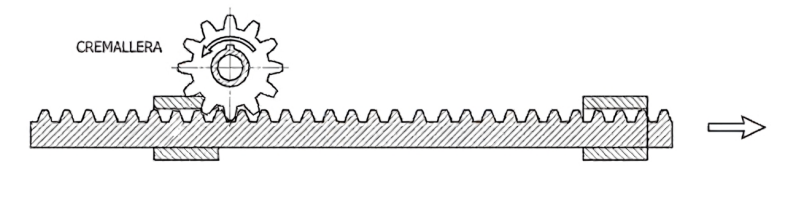
\includegraphics[width=\columnwidth]{img/cremallera.png}
    \caption{Alternativa piñon-cremallera}
    \label{fig:prototipo}
\end{figure}


\begin{table}[H]
\centering
\caption{Evaluación del sistema neumático.}
\begin{tabularx}{\columnwidth}{|X|X|}
\hline
\rowcolor{green!20}
Ventajas & Desventajas\\
\hline
Alta relación potencia-peso &
Modelado dinámico complejo\\
\hline
Movimiento suave &
Posicionamiento menos preciso\\
\hline
Amplio uso industrial &
Requiere compresor y accesorios\\
\hline
&
Mayor costo de implementación\\
\hline
\end{tabularx}
\end{table}

\begin{figure}[H]
    \centering
    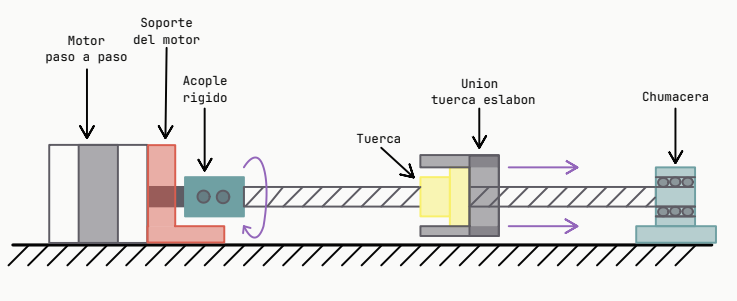
\includegraphics[width=\columnwidth]{img/tornillo.png}
    \caption{Alternativa tornillo-tuerca}
    \label{fig:prototipo_tornillo}
\end{figure}


Luego de analizar las tres alternativas y considerando criterios de precisión, facilidad de fabricación, costo y simplicidad de modelado, el equipo seleccionó el sistema tornillo-tuerca como mecanismo de accionamiento principal.

\subsubsection{Selección del material de las barras}

Para la fabricación de las barras del mecanismo se evaluaron diferentes materiales considerando criterios de masa, resistencia mecánica, facilidad de manufactura, disponibilidad comercial y costo.

\begin{table}[H]
\centering
\caption{Resultados de la votación para selección de material.}
\begin{tabularx}{\columnwidth}{|X|c|}
\hline
\rowcolor{gray!20}
Material & Votos\\
\hline
PVC & 2\\
Impresión 3D & 0\\
Acero & 0\\
Aluminio (varilla) & 3\\
Perfil de aluminio & 1\\
Acrílico & 3\\
\hline
\end{tabularx}
\end{table}

\begin{table}[H]
\centering
\caption{Evaluación técnica del aluminio.}
\begin{tabularx}{\columnwidth}{|X|X|}
\hline
\rowcolor{green!20}
Ventajas & Desventajas\\
\hline
Baja densidad &
Costo superior al PVC\\
\hline
Buena relación resistencia-peso &
Menor resistencia absoluta que el acero\\
\hline
Resistencia a la corrosión &
\\
\hline
Facilidad de mecanizado &
\\
\hline
Disponibilidad comercial &
\\
\hline
\end{tabularx}
\end{table}

Finalmente se seleccionó el aluminio debido a su favorable relación entre masa y resistencia mecánica, así como su apariencia profesional.

\subsubsection{Componentes seleccionados}

Una vez definidas las alternativas de diseño, se estableció la lista preliminar de componentes necesarios para la construcción del prototipo.

\begin{table}[H]
\centering
\caption{Componentes principales del sistema.}
\begin{tabularx}{\columnwidth}{|X|c|}
\hline
\rowcolor{gray!20}
Componente & Cantidad\\
\hline
Motor NEMA 17 & 2\\
Varilla roscada trapezoidal 8 mm & 2\\
Tuerca trapezoidal & 2\\
Guía lineal de aluminio & 2\\
Sensor BMI160 & 2\\
ESP32 & 1\\
\hline
\end{tabularx}
\end{table}

\subsubsection{Diseño asistido por computador}

El modelado tridimensional del sistema se desarrolló utilizando Autodesk Fusion 360. Esta herramienta permitió diseñar las piezas personalizadas, verificar interferencias geométricas y realizar el ensamblaje virtual previo a la fabricación física del mecanismo.

\subsection{Distribución de responsabilidades}

Con el fin de optimizar el desarrollo del proyecto, las actividades de diseño fueron distribuidas entre los integrantes del equipo.

\begin{table}[H]
\centering
\caption{Asignación de responsabilidades.}
\begin{tabularx}{\columnwidth}{|l|X|}
\hline
\rowcolor{gray!20}
Integrante & Actividad\\
\hline
David &
Diseño de uniones tuerca-varilla y soporte de sensores.\\
\hline
Sara &
Diseño de chumaceras y ensamblaje CAD.\\
\hline
Johel &
Diseño de la base y diagramas mecánicos.\\
\hline
Sergio &
Documentación en \LaTeX, rediseño del problema y soportes NEMA 17.\\
\hline
\end{tabularx}
\end{table}

\section{Descripción del prototipo seleccionado}

El prototipo desarrollado corresponde a la implementación física del mecanismo estudiado, compuesto por dos actuadores lineales ubicados en los puntos extremos y un sistema de barras articuladas que reproduce la configuración cinemática planteada inicialmente.



El movimiento vertical de los puntos A y C se genera mediante dos mecanismos independientes de tornillo-tuerca accionados por motores paso a paso NEMA 17. La rotación de cada motor se transforma en un desplazamiento lineal gracias a las varillas roscadas trapezoidales, permitiendo controlar la posición de los extremos del mecanismo con una relación geométrica conocida.

Las barras que conforman los eslabones móviles fueron fabricadas en aluminio, material seleccionado por su baja masa, adecuada rigidez estructural y facilidad de manufactura. Los puntos de unión se implementaron mediante articulaciones que permiten la rotación relativa entre los elementos, aproximando las condiciones ideales consideradas en el análisis teórico.

Para la adquisición de datos experimentales se incorporaron sensores inerciales BMI160, conectados a un microcontrolador ESP32 encargado de la lectura, procesamiento y transmisión de la información obtenida durante las pruebas. Esta instrumentación permite registrar las aceleraciones del mecanismo y compararlas posteriormente con los resultados obtenidos mediante el modelo dinámico.

Todos los componentes fueron montados sobre una base rígida (MDF). Adicionalmente, el ensamblaje completo fue modelado previamente en Autodesk Fusion 360 e Inventor, permitiendo verificar interferencias geométricas y validar el diseño antes de su fabricación.

\subsection{Principio de funcionamiento}

El funcionamiento del prototipo se basa en la conversión de movimiento rotacional a movimiento lineal mediante mecanismos tornillo-tuerca. Al girar los motores paso a paso, las tuercas acopladas a las varillas roscadas se desplazan verticalmente, generando el movimiento de los puntos A y C. Debido a la restricción impuesta por las barras articuladas, el punto B describe una trayectoria determinada por la geometría del mecanismo.
  % Eliminada inclusión recursiva (causaba bucle)
\subsection{Cinemática básica}
La cinemática es la parte de la mecánica que estudia el movimiento de los cuerpos sin
preocuparse por qué lo causan, es decir, sin importar fuerzas ni masas. Lo que interesa
aquí son las variables geométricas: posición, velocidad y aceleración en función del tiempo.
\\
\subsubsection{Posición y desplazamiento}

La posición de un punto en el plano se describe con un vector $\vec{r}$ que va desde el
origen del sistema de referencia hasta ese punto:

\begin{equation}
	\vec{r} = x\,\hat{i} + y\,\hat{j}
\end{equation}

El desplazamiento entre dos posiciones es simplemente la diferencia:

\begin{equation}
	\Delta\vec{r} = \vec{r}_2 - \vec{r}_1 = (x_2 - x_1)\,\hat{i} + (y_2 - y_1)\,\hat{j}
\end{equation}

En el mecanismo, los puntos $A$, $B$ y $C$ se ubican así en el plano. El punto $B$ es el
que queremos encontrar a partir de las posiciones que los actuadores imponen en $A$ y $C$.
\\
\subsubsection{Velocidad}

La velocidad es la derivada de la posición respecto al tiempo:

\begin{equation}
	\vec{v} = \frac{d\vec{r}}{dt} = \dot{x}\,\hat{i} + \dot{y}\,\hat{j}
\end{equation}

Su magnitud (la rapidez) es:

\begin{equation}
	|\vec{v}| = \sqrt{v_x^2 + v_y^2}
\end{equation}

En nuestro caso, las velocidades de $A$ y $C$ son conocidas y verticales:
$\vec{v}_A = 20\,\text{mm/s}\,\hat{j}$ y $\vec{v}_C = 30\,\text{mm/s}\,\hat{j}$.
Lo que se quiere encontrar es $\vec{v}_B$.

\subsubsection{Aceleración}

La aceleración es la derivada de la velocidad:

\begin{equation}
	\vec{a} = \frac{d\vec{v}}{dt} = \ddot{x}\,\hat{i} + \ddot{y}\,\hat{j}
\end{equation}

Cuando un punto describe una trayectoria curvilínea, la aceleración tiene dos componentes:
una tangencial (que cambia qué tan rápido va) y una normal o centrípeta (que cambia hacia
dónde va):

\begin{equation}
	\vec{a} = a_t\,\hat{e}_t + a_n\,\hat{e}_n
\end{equation}

La componente centrípeta para movimiento circular vale:

\begin{equation}
	a_n = \omega^2 \cdot r
\end{equation}

donde $\omega$ es la velocidad angular y $r$ la distancia al centro de rotación.
Esto aplica directamente al punto $B$, que sigue una trayectoria curvilínea al estar
conectado a los dos eslabones.

% ------------------------------------------------
\subsection{Cinemática de cuerpos rígidos}

Un cuerpo rígido es aquel en el que la distancia entre cualquier par de sus puntos no
cambia durante el movimiento. Gracias a esto, se puede extender el análisis de una partícula
a todo el cuerpo usando unas pocas ecuaciones.
\\
\subsubsection{Movimiento plano general}

El movimiento plano de un cuerpo rígido siempre se puede separar en una traslación (que
lleva un punto de referencia a su nueva posición) más una rotación alrededor de ese punto.
En general:

\begin{align} 
	\vec{r}_B &= \vec{r}_A + \vec{r}_{B/A} \label{eq:pos_rel} \\
	\vec{v}_B &= \vec{v}_A + \vec{v}_{B/A} \label{eq:vel_rel} \\
	\vec{a}_B &= \vec{a}_A + \vec{a}_{B/A} \label{eq:acc_rel} 
\end{align}

\subsubsection{Ecuación de velocidad relativa}

La velocidad de $B$ relativa a $A$, cuando el cuerpo rota con velocidad angular $\omega$,
se calcula con el producto vectorial:

\begin{equation}
	\vec{v}_{B/A} = \vec{\omega} \times \vec{r}_{B/A}
\end{equation}

Con $\vec{\omega} = \omega\,\hat{k}$ y $\vec{r}_{B/A} = r_x\,\hat{i} + r_y\,\hat{j}$,
el resultado en el plano es:

\begin{equation}
	\vec{v}_{B/A} = -\omega r_y\,\hat{i} + \omega r_x\,\hat{j}
\end{equation}

Aplicada al eslabón $CB$ del mecanismo:

\begin{equation}
	\vec{v}_B = \vec{v}_C + \vec{\omega}_{BC} \times \vec{r}_{B/C}
	\label{eq:vel_eslabon}
\end{equation}

Esta ecuación vectorial equivale a dos ecuaciones escalares (componentes $x$ e $y$), con
las que se pueden encontrar las dos incógnitas: las componentes de $\vec{v}_B$ y la
velocidad angular $\omega_{BC}$.
\\
\subsubsection{Ecuación de aceleración relativa}

La aceleración relativa tiene dos partes: la tangencial (por cambio en $\omega$) y la
centrípeta (por cambio de dirección):

\begin{equation}
	\vec{a}_{B/A} = \vec{\alpha} \times \vec{r}_{B/A} - \omega^2\,\vec{r}_{B/A}
\end{equation}

donde $\alpha = \dot{\omega}$ es la aceleración angular. La aceleración total de $B$ queda:

\begin{equation}
	\vec{a}_B = \vec{a}_A + \vec{\alpha} \times \vec{r}_{B/A} - \omega^2\,\vec{r}_{B/A}
\end{equation}

Para el eslabón $CB$:

\begin{equation}
	\vec{a}_B = \vec{a}_C + \alpha_{BC}\,\hat{k} \times \vec{r}_{B/C}
	- \omega_{BC}^2\,\vec{r}_{B/C}
	\label{eq:acc_eslabon}
\end{equation}

De nuevo, dos ecuaciones escalares que permiten hallar $\vec{a}_B$ y $\alpha_{BC}$,
una vez conocida $\omega_{BC}$ del paso anterior.
\\
\subsubsection{Lazo vectorial de cierre}

Para encontrar la posición de $B$ a partir de la geometría del mecanismo, se plantea
la ecuación de cierre del lazo:

\begin{equation}
	\vec{r}_B = \vec{r}_C + \vec{r}_{B/C} = \vec{r}_A + \vec{r}_{B/A}
\end{equation}

junto con las restricciones de longitud de cada eslabón:

\begin{align}
	|\vec{r}_{B/C}| &= b = 250\,\text{mm} \\
	|\vec{r}_{B/A}| &= a = 200\,\text{mm}
\end{align}

Esto forma un sistema de dos ecuaciones con dos incógnitas ($x_B$, $y_B$) que tiene
solución única para una configuración dada del mecanismo.

% ------------------------------------------------
\subsection{Mecanismo tornillo-tuerca}

Para generar el movimiento lineal de los puntos $A$ y $C$ se optó por un mecanismo
tornillo-tuerca, dado que sus componentes (barra roscada, tuerca y motor) son fácilmente
conseguibles y ofrecen buena precisión sin necesidad de impresión 3D de piezas críticas.

El principio es simple: el motor hace girar la barra roscada, y la tuerca que no puede
girar porque está unida al eslabón avanza linealmente. La relación entre la velocidad
angular del motor $\omega_m$ y la velocidad lineal resultante $v_L$ es:

\begin{equation}
	v_L = \frac{\omega_m \cdot p}{2\pi}
\end{equation}

donde $p$ es el paso del tornillo (avance por vuelta). El par necesario para vencer una
carga axial $F$ con eficiencia $\eta$ es:

\begin{equation}
	T = \frac{F \cdot p}{2\pi\,\eta}
\end{equation}

% ------------------------------------------------
\subsection{Motor paso a paso NEMA 17}

El motor paso a paso es un motor eléctrico que no gira continuamente sino que avanza en
pasos discretos. Cada pulso eléctrico que recibe el driver hace que el rotor se mueva un
ángulo fijo, llamado ángulo de paso $\theta_s$. Para el NEMA 17 genérico usado en este
proyecto, el ángulo de paso típico es de $1.8°$, lo que equivale a 200 pasos por vuelta.

Esto lo hace ideal para este mecanismo porque permite controlar la posición y velocidad
del actuador de forma precisa sin necesidad de un sensor de posición adicional en el motor,
simplemente contando los pulsos enviados:

\begin{equation}
	\theta = N_{pasos} \cdot \theta_s = N_{pasos} \cdot 1.8°
\end{equation}

\begin{equation}
	v_L = \frac{f_{pulsos} \cdot p}{N_{pasos/rev}}
	= \frac{f_{pulsos} \cdot p}{200}
\end{equation}

donde $f_{pulsos}$ es la frecuencia de los pulsos enviados por el microcontrolador.

A diferencia de un motor DC convencional, el motor paso a paso no requiere retroalimentación
para mantener una velocidad constante en régimen normal, ya que sigue fielmente los pulsos
de entrada siempre que la carga no supere el par de retención. Esto simplifica considerablemente
el control del mecanismo.

% ------------------------------------------------
\subsection{Microcontrolador ESP32}

El ESP32 es el cerebro del sistema. Es un microcontrolador de doble núcleo de 240 MHz con
Wi-Fi y Bluetooth integrados, aunque en este proyecto se usa principalmente por su capacidad
de generar señales de control precisas y leer sensores en tiempo real.

Para controlar el motor NEMA 17 se usa la técnica STEP/DIR: el ESP32 envía pulsos digitales
al driver del motor (por ejemplo A4988 o DRV8825) a través del pin STEP, y define la
dirección de giro con el pin DIR. La frecuencia de los pulsos determina la velocidad:

\begin{equation}
	f_{STEP} = \frac{v_L \cdot N_{pasos/rev}}{p}
\end{equation}

El ESP32 también se encarga de leer los acelerómetros vía protocolo I2C y enviar los datos
al computador por comunicación serial (UART) para su posterior procesamiento en Python o MATLAB.

% ------------------------------------------------
\subsection{Acelerómetro BMI160}

El BMI160 es un sensor MEMS (Micro-Electro-Mechanical Systems) de 6 grados de libertad incluye un acelerómetro triaxial y un giroscopio triaxial en el mismo
chip. En este proyecto se usan dos unidades, uno en el punto $B$ y otro en un punto de
referencia, para medir las aceleraciones del mecanismo durante su movimiento.

Su principio de funcionamiento se basa en la deflexión de una masa sísmica microscópica.
Cuando el sensor experimenta una aceleración, la masa se desplaza respecto a la estructura
fija, y ese desplazamiento se convierte en una diferencia de capacitancia que el chip
transforma en un valor digital.

La aceleración medida en unidades digitales (LSB) se convierte a $\text{m/s}^2$ usando
la sensibilidad del sensor, que depende del rango de medición configurado:

\begin{equation}
	a = \frac{\text{valor}_{LSB}}{\text{Sensibilidad}} \cdot g
\end{equation}

Por ejemplo, con rango $\pm 2g$ la sensibilidad es de $16384\,\text{LSB}/g$, y con
$\pm 4g$ es de $8192\,\text{LSB}/g$. Para este mecanismo, dado que las aceleraciones
esperadas son bajas (del orden de pocos $\text{mm/s}^2$), se configura el rango más
sensible ($\pm 2g$) para maximizar la resolución de las mediciones.

La comunicación con el ESP32 se realiza por el bus I2C a una velocidad de hasta 400 kHz.
Como se usan dos BMI160 en el mismo bus, se configuran en direcciones I2C distintas
(0x68 y 0x69) conectando el pin SDO de cada uno a GND o VDD respectivamente.

% ------------------------------------------------
\subsection{Circuito electrónico}

El circuito del prototipo se organiza en tres etapas: control, adquisición de datos y
potencia.
\subsubsection{Etapa de potencia -- Driver del motor paso a paso}

El motor NEMA 17 no se conecta directamente al ESP32 porque requiere corrientes del orden
de 1 A por fase, mucho más de lo que puede entregar un microcontrolador. Por eso se usa
un driver dedicado (A4988 o DRV8825) que actúa como interfaz entre los pulsos lógicos
del ESP32 y la corriente de las bobinas del motor.

El driver regula la corriente máxima por fase mediante un potenciómetro de ajuste. La
corriente de referencia $I_{ref}$ se relaciona con el voltaje en ese pin según:

\begin{equation}
	I_{ref} = \frac{V_{ref}}{8 \cdot R_{sense}} \quad \text{(para A4988)}
\end{equation}

donde $R_{sense}$ es la resistencia de detección de corriente del driver (típicamente
$0.1\,\Omega$ en módulos comerciales).
\subsubsection{Etapa lógica -- Conexiones del ESP32}

El ESP32 opera a 3.3 V en sus pines GPIO, lo cual es directamente compatible con los
niveles lógicos del driver de motor y del BMI160. Las conexiones principales son:

\begin{itemize}
	\item \textbf{STEP / DIR} del driver: conectados a dos GPIO del ESP32 por cada motor.
	\item \textbf{SDA / SCL} (I2C): bus compartido entre los dos BMI160 y el ESP32
	(pines GPIO 21 y GPIO 22 por defecto en ESP32).
	\item \textbf{ENABLE} del driver: activo en bajo; se mantiene en LOW para habilitar
	el motor durante la operación.
\end{itemize}
\subsubsection{Alimentación}


El circuito necesita dos niveles de tensión:

\begin{itemize}
	\item $3.3\,\text{V}$ para el ESP32 y los sensores BMI160 (regulado internamente
	por el módulo ESP32).
	\item $12\,\text{V}$ (o el voltaje nominal del NEMA 17) para la etapa de potencia
	del driver.
\end{itemize}

Es importante separar las masas de referencia de ambas etapas, o al menos usar un plano
de masa común bien conectado, para evitar que el ruido eléctrico de la conmutación del
motor afecte las lecturas del acelerómetro.

% Sección incluida ya en main.tex; comentar para evitar duplicado de etiquetas
% \section{Metodologías}
\subsection{Metodología de Diseño}

El desarrollo del mecanismo se llevó a cabo mediante una metodología  basada en reuniones periódicas del equipo, durante las cuales se evaluaron diferentes alternativas de diseño mecánico, electrónico y estructural. Cada decisión fue sustentada mediante criterios técnicos y posteriormente validada mediante votación entre los integrantes del grupo.

Inicialmente se analizó el mecanismo propuesto por el docente, identificando las variables cinemáticas y dinámicas involucradas, así como los requerimientos de medición necesarios para la adquisición de datos experimentales.

\subsubsection{Selección del sistema de medición}

Con el objetivo de registrar las aceleraciones presentes en el mecanismo, se evaluaron dos alternativas de sensores inerciales: el MPU6050 y el BMI160. La comparación se realizó considerando aspectos relevantes para la adquisición experimental de datos dinámicos.

\begin{table}[H]
\centering
\caption{Comparación entre sensores inerciales.}
\begin{tabularx}{\columnwidth}{|X|c|c|}
\hline
\rowcolor{gray!20}
Característica & MPU6050 & BMI160\\
\hline
Consumo energético & Alto & Bajo\\
Resolución acelerómetro & 14 bits & 16 bits\\
Resolución giroscopio & 16 bits & 16 bits\\
Tamaño FIFO & 512 bytes & 1024 bytes\\
Ruido de medición & Mayor & Menor\\
Modos de bajo consumo & Limitados & Avanzados\\
Tamaño físico & Mayor & Menor\\
\hline
\end{tabularx}
\end{table}

Tras la discusión técnica y posterior votación del equipo, se seleccionó el sensor BMI160 debido a su menor consumo energético, mayor resolución y mejor desempeño en la adquisición de señales dinámicas

\subsubsection{Selección del mecanismo de accionamiento}

Posteriormente se analizaron tres posibles mecanismos para generar el movimiento vertical de los puntos A y C: sistema tornillo-tuerca, sistema cremallera-piñón y cilindro neumático.


\begin{table}[H]
\centering
\caption{Evaluación del sistema tornillo-tuerca.}
\begin{tabularx}{\columnwidth}{|X|X|}
\hline
\rowcolor{green!20}
Ventajas & Desventajas\\
\hline
Relación de transmisión precisa y fácilmente modelable &
Presencia de fricción significativa\\
\hline
Alta capacidad de carga axial &
Requiere lubricación periódica\\
\hline
Buena repetibilidad del movimiento &
Posibles holguras axiales\\
\hline
Integración sencilla con motores paso a paso &
Velocidad lineal limitada\\
\hline
\end{tabularx}
\end{table}


\begin{table}[H]
\centering
\caption{Evaluación del sistema cremallera-piñón.}
\begin{tabularx}{\columnwidth}{|X|X|}
\hline
\rowcolor{green!20}
Ventajas & Desventajas\\
\hline
Conversión directa entre movimiento rotacional y lineal &
Presencia de backlash\\
\hline
Alta velocidad de desplazamiento &
Menor precisión de posicionamiento\\
\hline
Fabricación relativamente sencilla &
Mayor desgaste de los dientes\\
\hline
Mantenimiento reducido &
Requiere alineación precisa\\
\hline
\end{tabularx}
\end{table}
\begin{figure}[H]
    \centering
    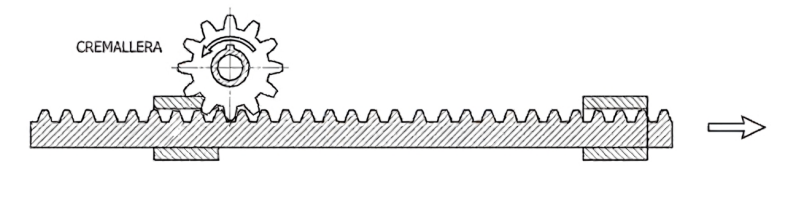
\includegraphics[width=\columnwidth]{img/cremallera.png}
    \caption{Alternativa piñon-cremallera}
    \label{fig:prototipo}
\end{figure}


\begin{table}[H]
\centering
\caption{Evaluación del sistema neumático.}
\begin{tabularx}{\columnwidth}{|X|X|}
\hline
\rowcolor{green!20}
Ventajas & Desventajas\\
\hline
Alta relación potencia-peso &
Modelado dinámico complejo\\
\hline
Movimiento suave &
Posicionamiento menos preciso\\
\hline
Amplio uso industrial &
Requiere compresor y accesorios\\
\hline
&
Mayor costo de implementación\\
\hline
\end{tabularx}
\end{table}

\begin{figure}[H]
    \centering
    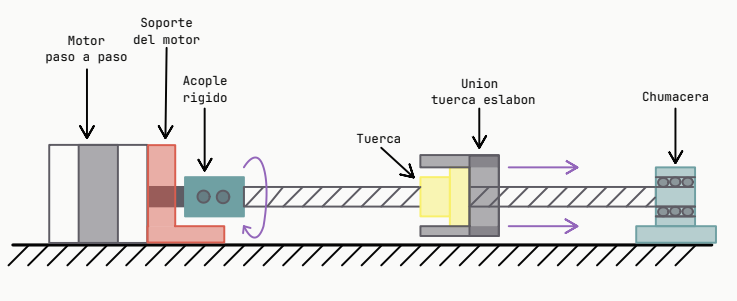
\includegraphics[width=\columnwidth]{img/tornillo.png}
    \caption{Alternativa tornillo-tuerca}
    \label{fig:prototipo_tornillo}
\end{figure}


Luego de analizar las tres alternativas y considerando criterios de precisión, facilidad de fabricación, costo y simplicidad de modelado, el equipo seleccionó el sistema tornillo-tuerca como mecanismo de accionamiento principal.

\subsubsection{Selección del material de las barras}

Para la fabricación de las barras del mecanismo se evaluaron diferentes materiales considerando criterios de masa, resistencia mecánica, facilidad de manufactura, disponibilidad comercial y costo.

\begin{table}[H]
\centering
\caption{Resultados de la votación para selección de material.}
\begin{tabularx}{\columnwidth}{|X|c|}
\hline
\rowcolor{gray!20}
Material & Votos\\
\hline
PVC & 2\\
Impresión 3D & 0\\
Acero & 0\\
Aluminio (varilla) & 3\\
Perfil de aluminio & 1\\
Acrílico & 3\\
\hline
\end{tabularx}
\end{table}

\begin{table}[H]
\centering
\caption{Evaluación técnica del aluminio.}
\begin{tabularx}{\columnwidth}{|X|X|}
\hline
\rowcolor{green!20}
Ventajas & Desventajas\\
\hline
Baja densidad &
Costo superior al PVC\\
\hline
Buena relación resistencia-peso &
Menor resistencia absoluta que el acero\\
\hline
Resistencia a la corrosión &
\\
\hline
Facilidad de mecanizado &
\\
\hline
Disponibilidad comercial &
\\
\hline
\end{tabularx}
\end{table}

Finalmente se seleccionó el aluminio debido a su favorable relación entre masa y resistencia mecánica, así como su apariencia profesional.

\subsubsection{Componentes seleccionados}

Una vez definidas las alternativas de diseño, se estableció la lista preliminar de componentes necesarios para la construcción del prototipo.

\begin{table}[H]
\centering
\caption{Componentes principales del sistema.}
\begin{tabularx}{\columnwidth}{|X|c|}
\hline
\rowcolor{gray!20}
Componente & Cantidad\\
\hline
Motor NEMA 17 & 2\\
Varilla roscada trapezoidal 8 mm & 2\\
Tuerca trapezoidal & 2\\
Guía lineal de aluminio & 2\\
Sensor BMI160 & 2\\
ESP32 & 1\\
\hline
\end{tabularx}
\end{table}

\subsubsection{Diseño asistido por computador}

El modelado tridimensional del sistema se desarrolló utilizando Autodesk Fusion 360. Esta herramienta permitió diseñar las piezas personalizadas, verificar interferencias geométricas y realizar el ensamblaje virtual previo a la fabricación física del mecanismo.

\subsection{Distribución de responsabilidades}

Con el fin de optimizar el desarrollo del proyecto, las actividades de diseño fueron distribuidas entre los integrantes del equipo.

\begin{table}[H]
\centering
\caption{Asignación de responsabilidades.}
\begin{tabularx}{\columnwidth}{|l|X|}
\hline
\rowcolor{gray!20}
Integrante & Actividad\\
\hline
David &
Diseño de uniones tuerca-varilla y soporte de sensores.\\
\hline
Sara &
Diseño de chumaceras y ensamblaje CAD.\\
\hline
Johel &
Diseño de la base y diagramas mecánicos.\\
\hline
Sergio &
Documentación en \LaTeX, rediseño del problema y soportes NEMA 17.\\
\hline
\end{tabularx}
\end{table}

\section{Descripción del prototipo seleccionado}

El prototipo desarrollado corresponde a la implementación física del mecanismo estudiado, compuesto por dos actuadores lineales ubicados en los puntos extremos y un sistema de barras articuladas que reproduce la configuración cinemática planteada inicialmente.



El movimiento vertical de los puntos A y C se genera mediante dos mecanismos independientes de tornillo-tuerca accionados por motores paso a paso NEMA 17. La rotación de cada motor se transforma en un desplazamiento lineal gracias a las varillas roscadas trapezoidales, permitiendo controlar la posición de los extremos del mecanismo con una relación geométrica conocida.

Las barras que conforman los eslabones móviles fueron fabricadas en aluminio, material seleccionado por su baja masa, adecuada rigidez estructural y facilidad de manufactura. Los puntos de unión se implementaron mediante articulaciones que permiten la rotación relativa entre los elementos, aproximando las condiciones ideales consideradas en el análisis teórico.

Para la adquisición de datos experimentales se incorporaron sensores inerciales BMI160, conectados a un microcontrolador ESP32 encargado de la lectura, procesamiento y transmisión de la información obtenida durante las pruebas. Esta instrumentación permite registrar las aceleraciones del mecanismo y compararlas posteriormente con los resultados obtenidos mediante el modelo dinámico.

Todos los componentes fueron montados sobre una base rígida (MDF). Adicionalmente, el ensamblaje completo fue modelado previamente en Autodesk Fusion 360 e Inventor, permitiendo verificar interferencias geométricas y validar el diseño antes de su fabricación.

\subsection{Principio de funcionamiento}

El funcionamiento del prototipo se basa en la conversión de movimiento rotacional a movimiento lineal mediante mecanismos tornillo-tuerca. Al girar los motores paso a paso, las tuercas acopladas a las varillas roscadas se desplazan verticalmente, generando el movimiento de los puntos A y C. Debido a la restricción impuesta por las barras articuladas, el punto B describe una trayectoria determinada por la geometría del mecanismo.
  % Eliminada inclusión recursiva (causaba bucle)
\subsection{Cinemática básica}
La cinemática es la parte de la mecánica que estudia el movimiento de los cuerpos sin
preocuparse por qué lo causan, es decir, sin importar fuerzas ni masas. Lo que interesa
aquí son las variables geométricas: posición, velocidad y aceleración en función del tiempo.
\\
\subsubsection{Posición y desplazamiento}

La posición de un punto en el plano se describe con un vector $\vec{r}$ que va desde el
origen del sistema de referencia hasta ese punto:

\begin{equation}
	\vec{r} = x\,\hat{i} + y\,\hat{j}
\end{equation}

El desplazamiento entre dos posiciones es simplemente la diferencia:

\begin{equation}
	\Delta\vec{r} = \vec{r}_2 - \vec{r}_1 = (x_2 - x_1)\,\hat{i} + (y_2 - y_1)\,\hat{j}
\end{equation}

En el mecanismo, los puntos $A$, $B$ y $C$ se ubican así en el plano. El punto $B$ es el
que queremos encontrar a partir de las posiciones que los actuadores imponen en $A$ y $C$.
\\
\subsubsection{Velocidad}

La velocidad es la derivada de la posición respecto al tiempo:

\begin{equation}
	\vec{v} = \frac{d\vec{r}}{dt} = \dot{x}\,\hat{i} + \dot{y}\,\hat{j}
\end{equation}

Su magnitud (la rapidez) es:

\begin{equation}
	|\vec{v}| = \sqrt{v_x^2 + v_y^2}
\end{equation}

En nuestro caso, las velocidades de $A$ y $C$ son conocidas y verticales:
$\vec{v}_A = 20\,\text{mm/s}\,\hat{j}$ y $\vec{v}_C = 30\,\text{mm/s}\,\hat{j}$.
Lo que se quiere encontrar es $\vec{v}_B$.

\subsubsection{Aceleración}

La aceleración es la derivada de la velocidad:

\begin{equation}
	\vec{a} = \frac{d\vec{v}}{dt} = \ddot{x}\,\hat{i} + \ddot{y}\,\hat{j}
\end{equation}

Cuando un punto describe una trayectoria curvilínea, la aceleración tiene dos componentes:
una tangencial (que cambia qué tan rápido va) y una normal o centrípeta (que cambia hacia
dónde va):

\begin{equation}
	\vec{a} = a_t\,\hat{e}_t + a_n\,\hat{e}_n
\end{equation}

La componente centrípeta para movimiento circular vale:

\begin{equation}
	a_n = \omega^2 \cdot r
\end{equation}

donde $\omega$ es la velocidad angular y $r$ la distancia al centro de rotación.
Esto aplica directamente al punto $B$, que sigue una trayectoria curvilínea al estar
conectado a los dos eslabones.

% ------------------------------------------------
\subsection{Cinemática de cuerpos rígidos}

Un cuerpo rígido es aquel en el que la distancia entre cualquier par de sus puntos no
cambia durante el movimiento. Gracias a esto, se puede extender el análisis de una partícula
a todo el cuerpo usando unas pocas ecuaciones.
\\
\subsubsection{Movimiento plano general}

El movimiento plano de un cuerpo rígido siempre se puede separar en una traslación (que
lleva un punto de referencia a su nueva posición) más una rotación alrededor de ese punto.
En general:

\begin{align} 
	\vec{r}_B &= \vec{r}_A + \vec{r}_{B/A} \label{eq:pos_rel} \\
	\vec{v}_B &= \vec{v}_A + \vec{v}_{B/A} \label{eq:vel_rel} \\
	\vec{a}_B &= \vec{a}_A + \vec{a}_{B/A} \label{eq:acc_rel} 
\end{align}

\subsubsection{Ecuación de velocidad relativa}

La velocidad de $B$ relativa a $A$, cuando el cuerpo rota con velocidad angular $\omega$,
se calcula con el producto vectorial:

\begin{equation}
	\vec{v}_{B/A} = \vec{\omega} \times \vec{r}_{B/A}
\end{equation}

Con $\vec{\omega} = \omega\,\hat{k}$ y $\vec{r}_{B/A} = r_x\,\hat{i} + r_y\,\hat{j}$,
el resultado en el plano es:

\begin{equation}
	\vec{v}_{B/A} = -\omega r_y\,\hat{i} + \omega r_x\,\hat{j}
\end{equation}

Aplicada al eslabón $CB$ del mecanismo:

\begin{equation}
	\vec{v}_B = \vec{v}_C + \vec{\omega}_{BC} \times \vec{r}_{B/C}
	\label{eq:vel_eslabon}
\end{equation}

Esta ecuación vectorial equivale a dos ecuaciones escalares (componentes $x$ e $y$), con
las que se pueden encontrar las dos incógnitas: las componentes de $\vec{v}_B$ y la
velocidad angular $\omega_{BC}$.
\\
\subsubsection{Ecuación de aceleración relativa}

La aceleración relativa tiene dos partes: la tangencial (por cambio en $\omega$) y la
centrípeta (por cambio de dirección):

\begin{equation}
	\vec{a}_{B/A} = \vec{\alpha} \times \vec{r}_{B/A} - \omega^2\,\vec{r}_{B/A}
\end{equation}

donde $\alpha = \dot{\omega}$ es la aceleración angular. La aceleración total de $B$ queda:

\begin{equation}
	\vec{a}_B = \vec{a}_A + \vec{\alpha} \times \vec{r}_{B/A} - \omega^2\,\vec{r}_{B/A}
\end{equation}

Para el eslabón $CB$:

\begin{equation}
	\vec{a}_B = \vec{a}_C + \alpha_{BC}\,\hat{k} \times \vec{r}_{B/C}
	- \omega_{BC}^2\,\vec{r}_{B/C}
	\label{eq:acc_eslabon}
\end{equation}

De nuevo, dos ecuaciones escalares que permiten hallar $\vec{a}_B$ y $\alpha_{BC}$,
una vez conocida $\omega_{BC}$ del paso anterior.
\\
\subsubsection{Lazo vectorial de cierre}

Para encontrar la posición de $B$ a partir de la geometría del mecanismo, se plantea
la ecuación de cierre del lazo:

\begin{equation}
	\vec{r}_B = \vec{r}_C + \vec{r}_{B/C} = \vec{r}_A + \vec{r}_{B/A}
\end{equation}

junto con las restricciones de longitud de cada eslabón:

\begin{align}
	|\vec{r}_{B/C}| &= b = 250\,\text{mm} \\
	|\vec{r}_{B/A}| &= a = 200\,\text{mm}
\end{align}

Esto forma un sistema de dos ecuaciones con dos incógnitas ($x_B$, $y_B$) que tiene
solución única para una configuración dada del mecanismo.

% ------------------------------------------------
\subsection{Mecanismo tornillo-tuerca}

Para generar el movimiento lineal de los puntos $A$ y $C$ se optó por un mecanismo
tornillo-tuerca, dado que sus componentes (barra roscada, tuerca y motor) son fácilmente
conseguibles y ofrecen buena precisión sin necesidad de impresión 3D de piezas críticas.

El principio es simple: el motor hace girar la barra roscada, y la tuerca que no puede
girar porque está unida al eslabón avanza linealmente. La relación entre la velocidad
angular del motor $\omega_m$ y la velocidad lineal resultante $v_L$ es:

\begin{equation}
	v_L = \frac{\omega_m \cdot p}{2\pi}
\end{equation}

donde $p$ es el paso del tornillo (avance por vuelta). El par necesario para vencer una
carga axial $F$ con eficiencia $\eta$ es:

\begin{equation}
	T = \frac{F \cdot p}{2\pi\,\eta}
\end{equation}

% ------------------------------------------------
\subsection{Motor paso a paso NEMA 17}

El motor paso a paso es un motor eléctrico que no gira continuamente sino que avanza en
pasos discretos. Cada pulso eléctrico que recibe el driver hace que el rotor se mueva un
ángulo fijo, llamado ángulo de paso $\theta_s$. Para el NEMA 17 genérico usado en este
proyecto, el ángulo de paso típico es de $1.8°$, lo que equivale a 200 pasos por vuelta.

Esto lo hace ideal para este mecanismo porque permite controlar la posición y velocidad
del actuador de forma precisa sin necesidad de un sensor de posición adicional en el motor,
simplemente contando los pulsos enviados:

\begin{equation}
	\theta = N_{pasos} \cdot \theta_s = N_{pasos} \cdot 1.8°
\end{equation}

\begin{equation}
	v_L = \frac{f_{pulsos} \cdot p}{N_{pasos/rev}}
	= \frac{f_{pulsos} \cdot p}{200}
\end{equation}

donde $f_{pulsos}$ es la frecuencia de los pulsos enviados por el microcontrolador.

A diferencia de un motor DC convencional, el motor paso a paso no requiere retroalimentación
para mantener una velocidad constante en régimen normal, ya que sigue fielmente los pulsos
de entrada siempre que la carga no supere el par de retención. Esto simplifica considerablemente
el control del mecanismo.

% ------------------------------------------------
\subsection{Microcontrolador ESP32}

El ESP32 es el cerebro del sistema. Es un microcontrolador de doble núcleo de 240 MHz con
Wi-Fi y Bluetooth integrados, aunque en este proyecto se usa principalmente por su capacidad
de generar señales de control precisas y leer sensores en tiempo real.

Para controlar el motor NEMA 17 se usa la técnica STEP/DIR: el ESP32 envía pulsos digitales
al driver del motor (por ejemplo A4988 o DRV8825) a través del pin STEP, y define la
dirección de giro con el pin DIR. La frecuencia de los pulsos determina la velocidad:

\begin{equation}
	f_{STEP} = \frac{v_L \cdot N_{pasos/rev}}{p}
\end{equation}

El ESP32 también se encarga de leer los acelerómetros vía protocolo I2C y enviar los datos
al computador por comunicación serial (UART) para su posterior procesamiento en Python o MATLAB.

% ------------------------------------------------
\subsection{Acelerómetro BMI160}

El BMI160 es un sensor MEMS (Micro-Electro-Mechanical Systems) de 6 grados de libertad incluye un acelerómetro triaxial y un giroscopio triaxial en el mismo
chip. En este proyecto se usan dos unidades, uno en el punto $B$ y otro en un punto de
referencia, para medir las aceleraciones del mecanismo durante su movimiento.

Su principio de funcionamiento se basa en la deflexión de una masa sísmica microscópica.
Cuando el sensor experimenta una aceleración, la masa se desplaza respecto a la estructura
fija, y ese desplazamiento se convierte en una diferencia de capacitancia que el chip
transforma en un valor digital.

La aceleración medida en unidades digitales (LSB) se convierte a $\text{m/s}^2$ usando
la sensibilidad del sensor, que depende del rango de medición configurado:

\begin{equation}
	a = \frac{\text{valor}_{LSB}}{\text{Sensibilidad}} \cdot g
\end{equation}

Por ejemplo, con rango $\pm 2g$ la sensibilidad es de $16384\,\text{LSB}/g$, y con
$\pm 4g$ es de $8192\,\text{LSB}/g$. Para este mecanismo, dado que las aceleraciones
esperadas son bajas (del orden de pocos $\text{mm/s}^2$), se configura el rango más
sensible ($\pm 2g$) para maximizar la resolución de las mediciones.

La comunicación con el ESP32 se realiza por el bus I2C a una velocidad de hasta 400 kHz.
Como se usan dos BMI160 en el mismo bus, se configuran en direcciones I2C distintas
(0x68 y 0x69) conectando el pin SDO de cada uno a GND o VDD respectivamente.

% ------------------------------------------------
\subsection{Circuito electrónico}

El circuito del prototipo se organiza en tres etapas: control, adquisición de datos y
potencia.
\subsubsection{Etapa de potencia -- Driver del motor paso a paso}

El motor NEMA 17 no se conecta directamente al ESP32 porque requiere corrientes del orden
de 1 A por fase, mucho más de lo que puede entregar un microcontrolador. Por eso se usa
un driver dedicado (A4988 o DRV8825) que actúa como interfaz entre los pulsos lógicos
del ESP32 y la corriente de las bobinas del motor.

El driver regula la corriente máxima por fase mediante un potenciómetro de ajuste. La
corriente de referencia $I_{ref}$ se relaciona con el voltaje en ese pin según:

\begin{equation}
	I_{ref} = \frac{V_{ref}}{8 \cdot R_{sense}} \quad \text{(para A4988)}
\end{equation}

donde $R_{sense}$ es la resistencia de detección de corriente del driver (típicamente
$0.1\,\Omega$ en módulos comerciales).
\subsubsection{Etapa lógica -- Conexiones del ESP32}

El ESP32 opera a 3.3 V en sus pines GPIO, lo cual es directamente compatible con los
niveles lógicos del driver de motor y del BMI160. Las conexiones principales son:

\begin{itemize}
	\item \textbf{STEP / DIR} del driver: conectados a dos GPIO del ESP32 por cada motor.
	\item \textbf{SDA / SCL} (I2C): bus compartido entre los dos BMI160 y el ESP32
	(pines GPIO 21 y GPIO 22 por defecto en ESP32).
	\item \textbf{ENABLE} del driver: activo en bajo; se mantiene en LOW para habilitar
	el motor durante la operación.
\end{itemize}
\subsubsection{Alimentación}


El circuito necesita dos niveles de tensión:

\begin{itemize}
	\item $3.3\,\text{V}$ para el ESP32 y los sensores BMI160 (regulado internamente
	por el módulo ESP32).
	\item $12\,\text{V}$ (o el voltaje nominal del NEMA 17) para la etapa de potencia
	del driver.
\end{itemize}

Es importante separar las masas de referencia de ambas etapas, o al menos usar un plano
de masa común bien conectado, para evitar que el ruido eléctrico de la conmutación del
motor afecte las lecturas del acelerómetro.

% Sección incluida ya en main.tex; comentar para evitar duplicado de etiquetas
% \section{Metodologías}
\subsection{Metodología de Diseño}

El desarrollo del mecanismo se llevó a cabo mediante una metodología  basada en reuniones periódicas del equipo, durante las cuales se evaluaron diferentes alternativas de diseño mecánico, electrónico y estructural. Cada decisión fue sustentada mediante criterios técnicos y posteriormente validada mediante votación entre los integrantes del grupo.

Inicialmente se analizó el mecanismo propuesto por el docente, identificando las variables cinemáticas y dinámicas involucradas, así como los requerimientos de medición necesarios para la adquisición de datos experimentales.

\subsubsection{Selección del sistema de medición}

Con el objetivo de registrar las aceleraciones presentes en el mecanismo, se evaluaron dos alternativas de sensores inerciales: el MPU6050 y el BMI160. La comparación se realizó considerando aspectos relevantes para la adquisición experimental de datos dinámicos.

\begin{table}[H]
\centering
\caption{Comparación entre sensores inerciales.}
\begin{tabularx}{\columnwidth}{|X|c|c|}
\hline
\rowcolor{gray!20}
Característica & MPU6050 & BMI160\\
\hline
Consumo energético & Alto & Bajo\\
Resolución acelerómetro & 14 bits & 16 bits\\
Resolución giroscopio & 16 bits & 16 bits\\
Tamaño FIFO & 512 bytes & 1024 bytes\\
Ruido de medición & Mayor & Menor\\
Modos de bajo consumo & Limitados & Avanzados\\
Tamaño físico & Mayor & Menor\\
\hline
\end{tabularx}
\end{table}

Tras la discusión técnica y posterior votación del equipo, se seleccionó el sensor BMI160 debido a su menor consumo energético, mayor resolución y mejor desempeño en la adquisición de señales dinámicas

\subsubsection{Selección del mecanismo de accionamiento}

Posteriormente se analizaron tres posibles mecanismos para generar el movimiento vertical de los puntos A y C: sistema tornillo-tuerca, sistema cremallera-piñón y cilindro neumático.


\begin{table}[H]
\centering
\caption{Evaluación del sistema tornillo-tuerca.}
\begin{tabularx}{\columnwidth}{|X|X|}
\hline
\rowcolor{green!20}
Ventajas & Desventajas\\
\hline
Relación de transmisión precisa y fácilmente modelable &
Presencia de fricción significativa\\
\hline
Alta capacidad de carga axial &
Requiere lubricación periódica\\
\hline
Buena repetibilidad del movimiento &
Posibles holguras axiales\\
\hline
Integración sencilla con motores paso a paso &
Velocidad lineal limitada\\
\hline
\end{tabularx}
\end{table}


\begin{table}[H]
\centering
\caption{Evaluación del sistema cremallera-piñón.}
\begin{tabularx}{\columnwidth}{|X|X|}
\hline
\rowcolor{green!20}
Ventajas & Desventajas\\
\hline
Conversión directa entre movimiento rotacional y lineal &
Presencia de backlash\\
\hline
Alta velocidad de desplazamiento &
Menor precisión de posicionamiento\\
\hline
Fabricación relativamente sencilla &
Mayor desgaste de los dientes\\
\hline
Mantenimiento reducido &
Requiere alineación precisa\\
\hline
\end{tabularx}
\end{table}
\begin{figure}[H]
    \centering
    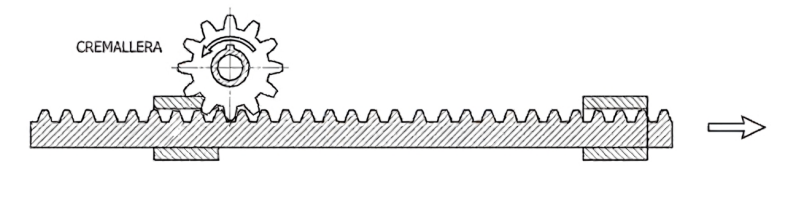
\includegraphics[width=\columnwidth]{img/cremallera.png}
    \caption{Alternativa piñon-cremallera}
    \label{fig:prototipo}
\end{figure}


\begin{table}[H]
\centering
\caption{Evaluación del sistema neumático.}
\begin{tabularx}{\columnwidth}{|X|X|}
\hline
\rowcolor{green!20}
Ventajas & Desventajas\\
\hline
Alta relación potencia-peso &
Modelado dinámico complejo\\
\hline
Movimiento suave &
Posicionamiento menos preciso\\
\hline
Amplio uso industrial &
Requiere compresor y accesorios\\
\hline
&
Mayor costo de implementación\\
\hline
\end{tabularx}
\end{table}

\begin{figure}[H]
    \centering
    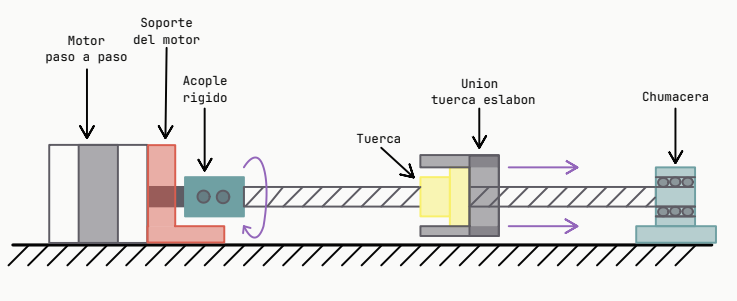
\includegraphics[width=\columnwidth]{img/tornillo.png}
    \caption{Alternativa tornillo-tuerca}
    \label{fig:prototipo_tornillo}
\end{figure}


Luego de analizar las tres alternativas y considerando criterios de precisión, facilidad de fabricación, costo y simplicidad de modelado, el equipo seleccionó el sistema tornillo-tuerca como mecanismo de accionamiento principal.

\subsubsection{Selección del material de las barras}

Para la fabricación de las barras del mecanismo se evaluaron diferentes materiales considerando criterios de masa, resistencia mecánica, facilidad de manufactura, disponibilidad comercial y costo.

\begin{table}[H]
\centering
\caption{Resultados de la votación para selección de material.}
\begin{tabularx}{\columnwidth}{|X|c|}
\hline
\rowcolor{gray!20}
Material & Votos\\
\hline
PVC & 2\\
Impresión 3D & 0\\
Acero & 0\\
Aluminio (varilla) & 3\\
Perfil de aluminio & 1\\
Acrílico & 3\\
\hline
\end{tabularx}
\end{table}

\begin{table}[H]
\centering
\caption{Evaluación técnica del aluminio.}
\begin{tabularx}{\columnwidth}{|X|X|}
\hline
\rowcolor{green!20}
Ventajas & Desventajas\\
\hline
Baja densidad &
Costo superior al PVC\\
\hline
Buena relación resistencia-peso &
Menor resistencia absoluta que el acero\\
\hline
Resistencia a la corrosión &
\\
\hline
Facilidad de mecanizado &
\\
\hline
Disponibilidad comercial &
\\
\hline
\end{tabularx}
\end{table}

Finalmente se seleccionó el aluminio debido a su favorable relación entre masa y resistencia mecánica, así como su apariencia profesional.

\subsubsection{Componentes seleccionados}

Una vez definidas las alternativas de diseño, se estableció la lista preliminar de componentes necesarios para la construcción del prototipo.

\begin{table}[H]
\centering
\caption{Componentes principales del sistema.}
\begin{tabularx}{\columnwidth}{|X|c|}
\hline
\rowcolor{gray!20}
Componente & Cantidad\\
\hline
Motor NEMA 17 & 2\\
Varilla roscada trapezoidal 8 mm & 2\\
Tuerca trapezoidal & 2\\
Guía lineal de aluminio & 2\\
Sensor BMI160 & 2\\
ESP32 & 1\\
\hline
\end{tabularx}
\end{table}

\subsubsection{Diseño asistido por computador}

El modelado tridimensional del sistema se desarrolló utilizando Autodesk Fusion 360. Esta herramienta permitió diseñar las piezas personalizadas, verificar interferencias geométricas y realizar el ensamblaje virtual previo a la fabricación física del mecanismo.

\subsection{Distribución de responsabilidades}

Con el fin de optimizar el desarrollo del proyecto, las actividades de diseño fueron distribuidas entre los integrantes del equipo.

\begin{table}[H]
\centering
\caption{Asignación de responsabilidades.}
\begin{tabularx}{\columnwidth}{|l|X|}
\hline
\rowcolor{gray!20}
Integrante & Actividad\\
\hline
David &
Diseño de uniones tuerca-varilla y soporte de sensores.\\
\hline
Sara &
Diseño de chumaceras y ensamblaje CAD.\\
\hline
Johel &
Diseño de la base y diagramas mecánicos.\\
\hline
Sergio &
Documentación en \LaTeX, rediseño del problema y soportes NEMA 17.\\
\hline
\end{tabularx}
\end{table}

\section{Descripción del prototipo seleccionado}

El prototipo desarrollado corresponde a la implementación física del mecanismo estudiado, compuesto por dos actuadores lineales ubicados en los puntos extremos y un sistema de barras articuladas que reproduce la configuración cinemática planteada inicialmente.



El movimiento vertical de los puntos A y C se genera mediante dos mecanismos independientes de tornillo-tuerca accionados por motores paso a paso NEMA 17. La rotación de cada motor se transforma en un desplazamiento lineal gracias a las varillas roscadas trapezoidales, permitiendo controlar la posición de los extremos del mecanismo con una relación geométrica conocida.

Las barras que conforman los eslabones móviles fueron fabricadas en aluminio, material seleccionado por su baja masa, adecuada rigidez estructural y facilidad de manufactura. Los puntos de unión se implementaron mediante articulaciones que permiten la rotación relativa entre los elementos, aproximando las condiciones ideales consideradas en el análisis teórico.

Para la adquisición de datos experimentales se incorporaron sensores inerciales BMI160, conectados a un microcontrolador ESP32 encargado de la lectura, procesamiento y transmisión de la información obtenida durante las pruebas. Esta instrumentación permite registrar las aceleraciones del mecanismo y compararlas posteriormente con los resultados obtenidos mediante el modelo dinámico.

Todos los componentes fueron montados sobre una base rígida (MDF). Adicionalmente, el ensamblaje completo fue modelado previamente en Autodesk Fusion 360 e Inventor, permitiendo verificar interferencias geométricas y validar el diseño antes de su fabricación.

\subsection{Principio de funcionamiento}

El funcionamiento del prototipo se basa en la conversión de movimiento rotacional a movimiento lineal mediante mecanismos tornillo-tuerca. Al girar los motores paso a paso, las tuercas acopladas a las varillas roscadas se desplazan verticalmente, generando el movimiento de los puntos A y C. Debido a la restricción impuesta por las barras articuladas, el punto B describe una trayectoria determinada por la geometría del mecanismo.
